\documentclass[default,pdf,colorBG,slideColor]{prosper}
\usepackage{epsfig}
\usepackage{pstricks}
\usepackage{graphicx}

\graphicspath{ {../fig/} }

\title{Next Generation Resource Manager}
\subtitle{{\small high level technical review}}
\author{Dong Ahn, Jim Garlick, Mark Grondona, Don Lipari}
\email{{\rm \{ahn1,garlick,mgrondona,lipari\}@llnl.gov}}
\institution{Livermore Computing \\
             Lawrence Livermore National Laboratory}

\newcommand{\ngrm}{NGRM}
\newcommand{\zMQ}{\O{}MQ}

\slideCaption{\ngrm\ High Level Review, Mar. 4, 2013}

\Logo(-1,-1){
\epsfig{file=graphic/iccd_logotrans.ps,scale=0.15}}

%\Logo{
\includegraphics[scale=0.15]{iccd_logotrans.ps}}

\newif\ifbigpic
\bigpictrue


\begin{document}

% ==========================================================================
\maketitle
% ==========================================================================
\begin{slide}{Session Overview}{\small
We will roughly follow the outline of the {\em Vision} document.\\
\begin{itemize}
  \item[\S1-4]{{\em overview} (Jim)}
  \item[\S5]{{\em comms framework} (Jim)}
  \item[\S6.1-6]{{\em resource management} (Mark)}
  \item[\S6.7]{{\em scheduler} (Don)}
  \item[\S7]{{\em monitoring} (Jim)}
  \item[\S8]{{\em runtime} (Dong)}
\end{itemize}
We expect to address your questions and comments as we go.
}\end{slide}
% ==========================================================================
\part{overview}
% ==========================================================================
\begin{slide}{Emerging Challenges for RM}{\small
\begin{itemize}
  \item{extreme scalability}
  \item{low noise}
  \item{fault tolerance}
  \item{heterogeneity (GPUs, FPGA, special nodes)}
  \item{new resource types (power, I/O)}
  \item{code devel/debug complexity}
  \item{new workloads (high job throughput, UQ, exascale)}
\end{itemize}
Failure to adapt will harm user productivity.
}\end{slide}
% ==========================================================================
\begin{slide}{Could Slurm be Adapted?}{\small
We think not.
\begin{itemize}
  \item{older paradigm: monolithic controller, node-scheduled}
  \item{minimal runtime support (env vars, libslurm, libpmi, MPIR)}
  \item{scalability limitations}
  \item{comprehensive redesign overdue}
  \item{need center-wide RM to manage simulation ensembles, I/O, viz, etc}
\end{itemize}
}\end{slide}
% ==========================================================================
\begin{slide}{Vision and New Capabilities}{\small
\begin{itemize}
  \item{center as a cluster}
  \item{diverse compute resources}
  \item{data provenance and reproduceability}
  \item{low noise}
  \item{fault tolerance}
  \item{security}
  \item{research and tool friendly}
  \item{extensibility}
\end{itemize}
}\end{slide}
% ==========================================================================
\begin{slide}{Design Challenges}{\small
\begin{minipage}{0.47\textwidth}
\begin{itemize}
  \item{multidimensional scale}
  \item{diverse workload}
  \item{dynamic workload}
  \item{power}
  \item{scheduling}
\end{itemize}
\end{minipage}
\begin{minipage}{0.47\textwidth}
\begin{itemize}
  \item{backwards compatibility}
  \item{integration risk}
  \item{higher downtime costs}
  \item{separation-of-concerns}
  \item{security}
  \item{productivity}
\end{itemize}
\end{minipage}
}\end{slide}
% ==========================================================================
\begin{slide}{New Conceptual Models}{\small
\begin{itemize}
  \item{unified job $=$ resource allocation $+$ RM instance}
  \item{job hierarchy}
  \begin{itemize}
    \item{parent bounding rule}
    \item{child empowerment rule}
    \item{parental consent rule}
  \end{itemize}
  \item{generalized resource}
  \item{resource allocation elasticity}
  \item{common scalable infrastructure}
  \item{self-hosting}
  \item{lightweight virtualization}
\end{itemize}
}\end{slide}
% ==========================================================================
\begin{slide}{Resource Hierarchy}{\small
\ifbigpic
\begin{center}
  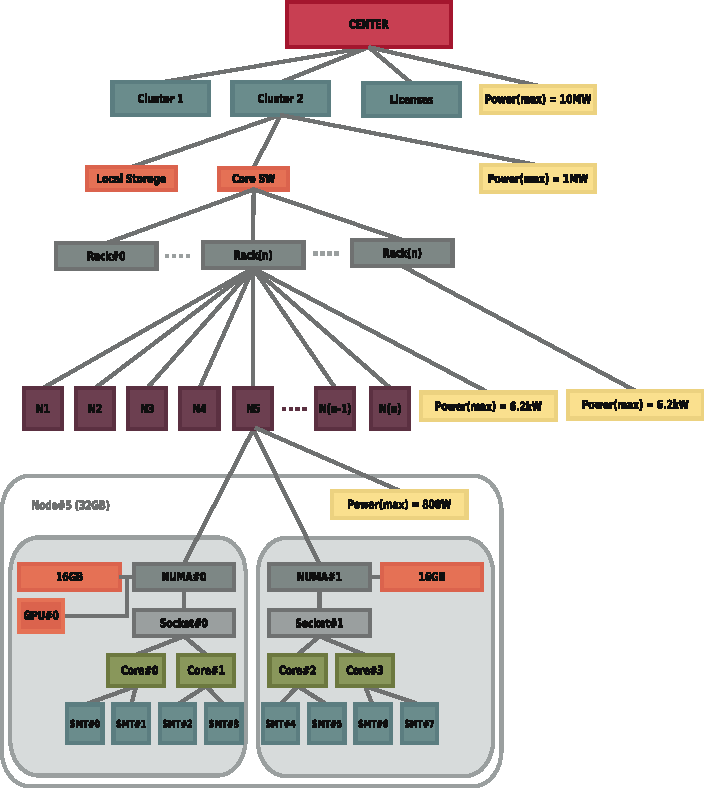
\includegraphics[scale=0.50]{resource-hierarchy}
\end{center}
\fi
}\end{slide}
% ==========================================================================
\begin{slide}{\ngrm\ Job Attributes (1/2)}{\small
\begin{itemize}
  \item{job owner and ACL users can run and/or submit jobs;\\
	owners can "invite" debug help or coordinate DAT}
  \item{RM instance with resource subset, topology, etc}
  \item{scheduler to accept and schedule new jobs,\\
	scheduler plugin selectable by owner}
  \item{job DB recording new, running, completed child jobs;\\
	job\&res DBs "reaped" like UNIX processes at job exit}
\end{itemize}
}\end{slide}
% ==========================================================================
\begin{slide}{\ngrm\ Job Attributes (2/2)}{\small
\begin{itemize}
  \item{isolated communications framework with parent gateway}
  \item{runtime environment for launching parallel apps \& tools}
  \item{interactive node for batch scripts/user logins}
  \item{resolvable domain name based on unique jobid,\\
	ssh to job, point web browser at job}
  \item{local monitoring domain, user configurable}
\end{itemize}
}\end{slide}
% ==========================================================================
\begin{slide}{Lightweight Jobs (LWJ)}{\small
\begin{itemize}
  \item{LWJ is a job sharing parent RM instance,
	communications framework, etc}
  \item{optimizes base case of allocate \& launch MPI job}
  \item{covers co-located work like tool processes}
  \item{regular jobs $\sim$ UNIX processes; LWJ $\sim$ UNIX threads}
\end{itemize}
}\end{slide}
% ==========================================================================
\begin{slide}{job 0 spans all resources}{\small
\ifbigpic
\begin{center}
  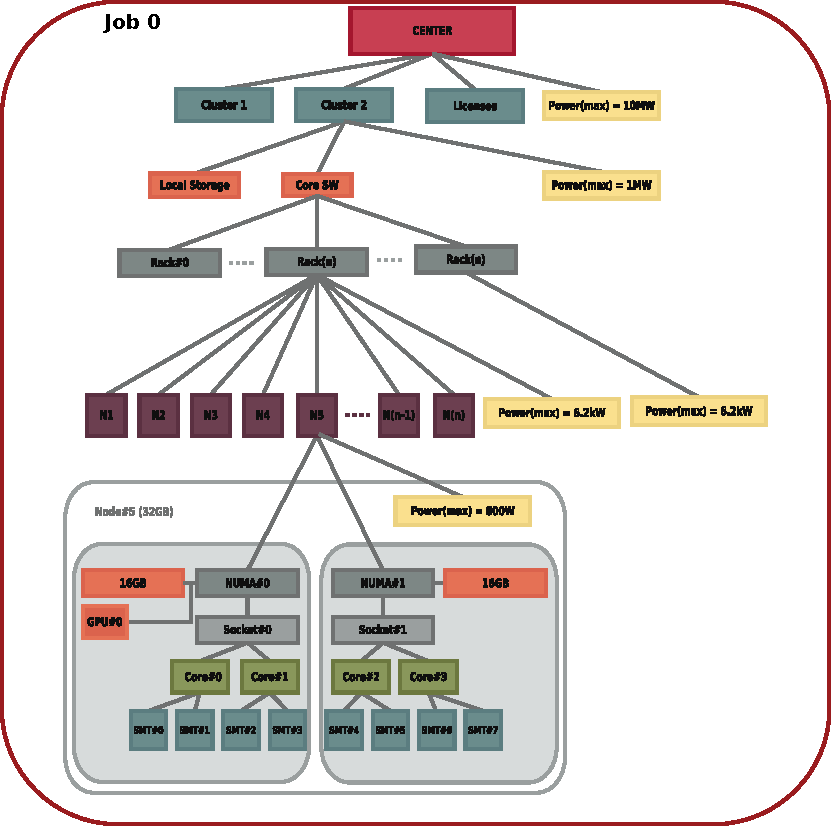
\includegraphics[scale=0.50]{job-hierarchy-job0}
\end{center}
\fi
}\end{slide}
% ==========================================================================
\begin{slide}{job 0.x on cluster 2}{\small
\ifbigpic
\begin{center}
  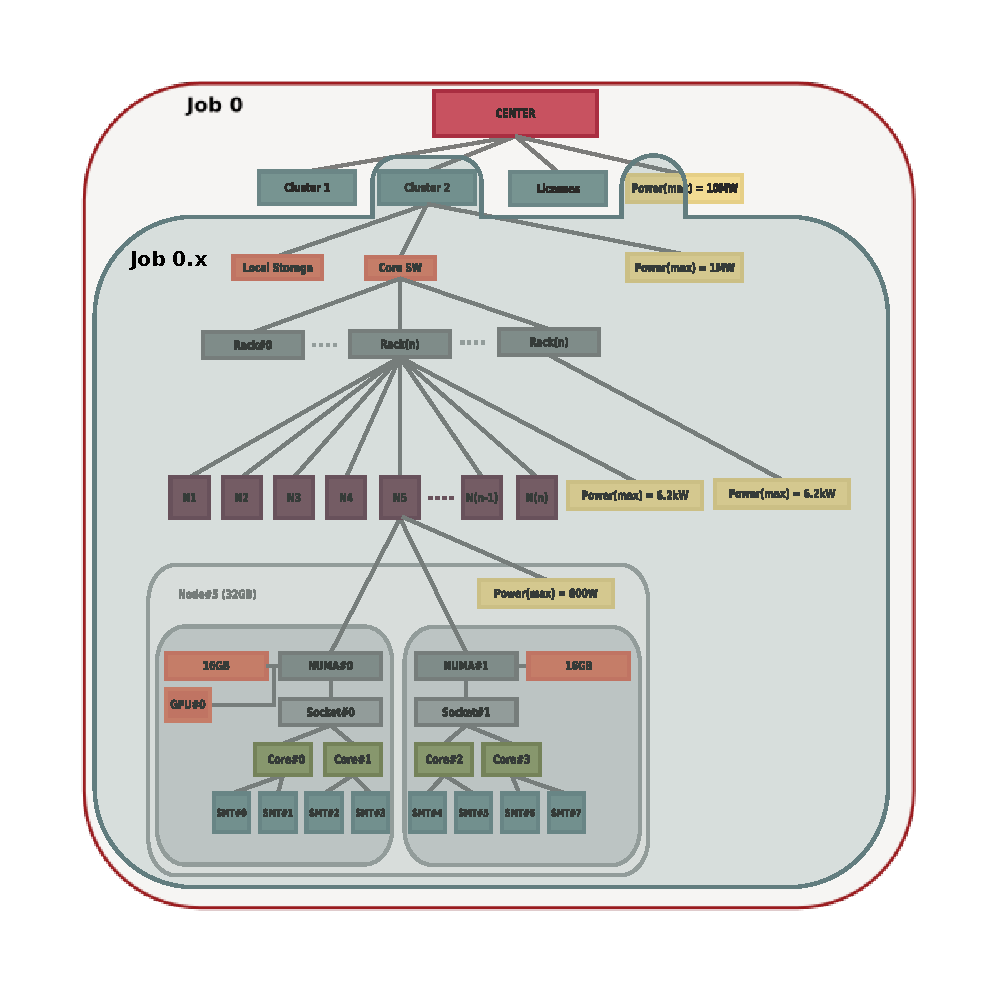
\includegraphics[scale=0.50]{job-hierarchy-job0-x}
\end{center}
\fi
}\end{slide}
% ==========================================================================
\begin{slide}{job 0.x.y on nodes n1-5}{\small
\ifbigpic
\begin{center}
  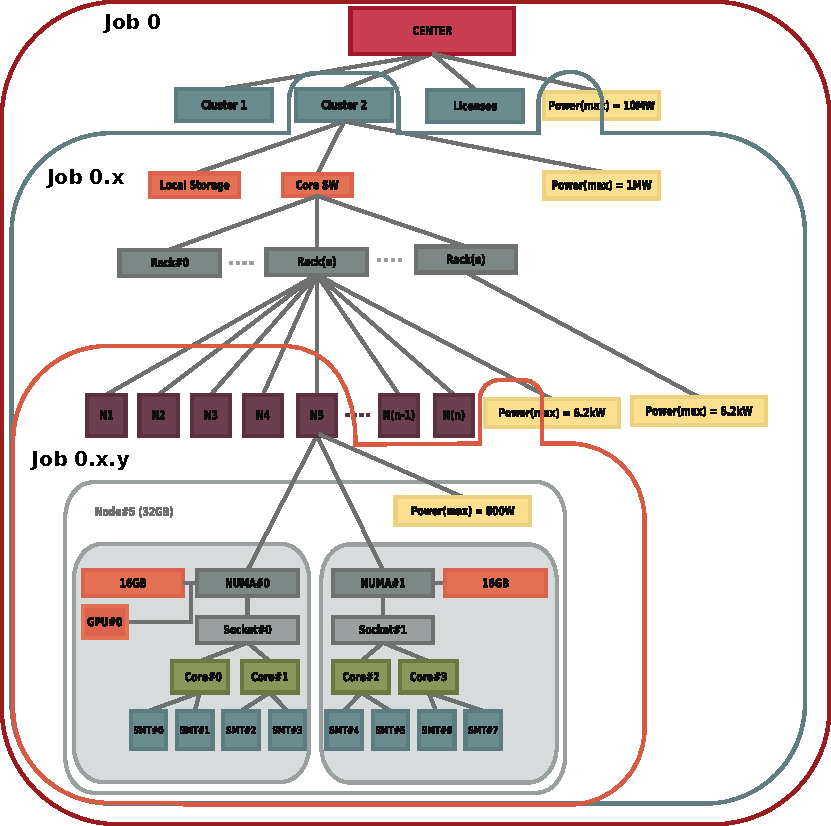
\includegraphics[scale=0.50]{job-hierarchy-job0-x-y}
\end{center}
\fi
}\end{slide}
% ==========================================================================
\begin{slide}{2 LWJs on node n5}{\small
\ifbigpic
\begin{center}
  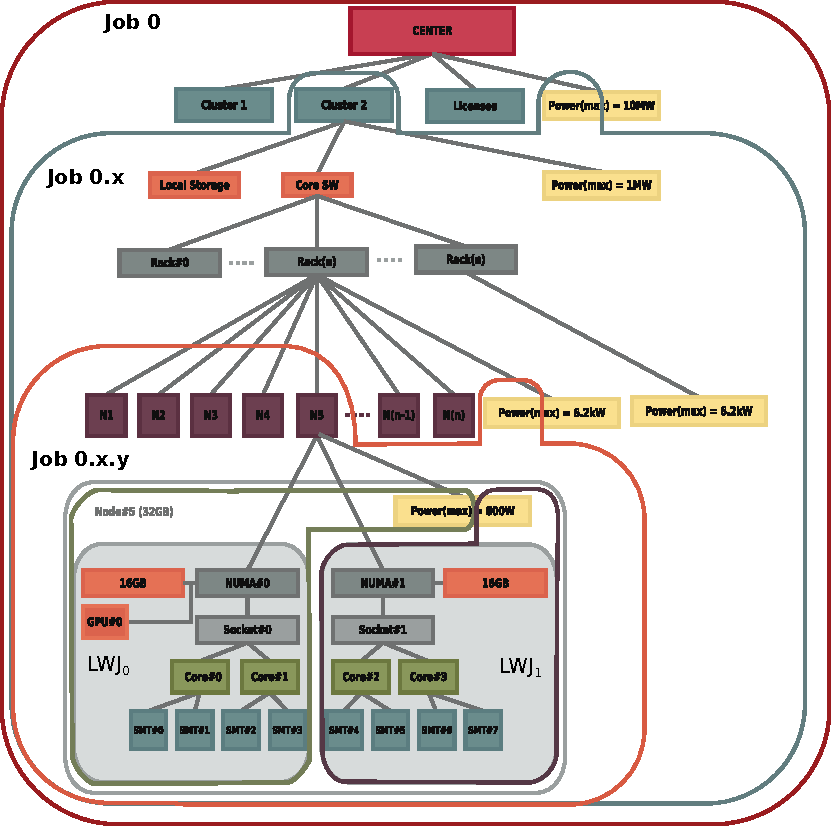
\includegraphics[scale=0.50]{job-hierarchy-lwj}
\end{center}
\fi
}\end{slide}
% ==========================================================================
\begin{slide}{Project Thrust Areas}{\small
\textbf{Comms Framework:}
    common scalable infrastrucure model for \ngrm\ components\\
\vspace{0.5cm}
\textbf{Resource Management:}
    config, scheduling, tracking of resources, jobs and users\\
\vspace{0.5cm}
\textbf{Monitoring:}
    scalable resource health monitoring, fault notification, logging\\
\vspace{0.5cm}
\textbf{Runtime:}
    support for application runtime, tools, process management, etc.
}\end{slide}
% ==========================================================================
\part{comms framework}
% ==========================================================================
\begin{slide}{Comms Framework Goals}{\small
\begin{itemize}
  \item{Build a foundation for \ngrm\ distributed components.}
  \item{A {\em comms session} contains each \ngrm\ job, and \\
	job hierarchy $\sim$ comms session hierarchy}
  \item{Rich comms within a session,\\
	No direct comms between sibling sessions,\\
        Limited comms between parent-child (through gateway)}
  \item{Parent session can create, resize, destroy child sessions}
  \item{Comms consists of four layers...}
\end{itemize}
}\end{slide}
% ==========================================================================
\begin{slide}{Comms Framework Layers}{\small
\begin{center}
  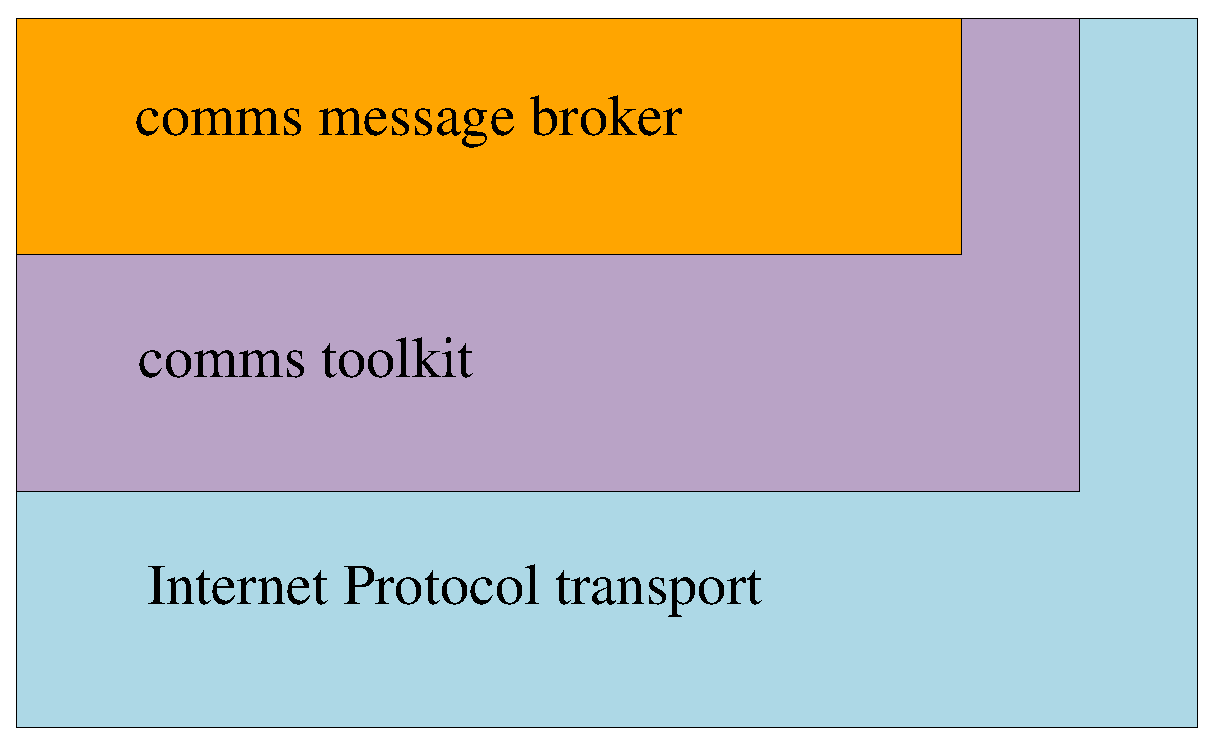
\includegraphics[scale=0.20]{comms}
\end{center}
\begin{itemize}
  \item{Layering is not rigid\\
        \ngrm\ components not overly constrained}
  \item{Bottom two layers are mostly off-the-shelf}
  \item{Generality reflects early phase of project in which it was conceived}
\end{itemize}
}\end{slide}
% ==========================================================================
\begin{slide}{Internet Protocols and Services}{\small
\begin{itemize}
  \item{Fully routed IP networks, e.g. route cluster management
	ethernets and IP-over-IB together}
  \item{Dynamic IP assignment, including multicast}
  \item{Private DNS, each session has a name, e.g. {\tt s2.s400.\ngrm.}}
  \item{Possibility for VPN isolation between jobs}
\end{itemize}
}\end{slide}
% ==========================================================================
\begin{slide}{Comms Toolkit}{\small
\begin{center}
  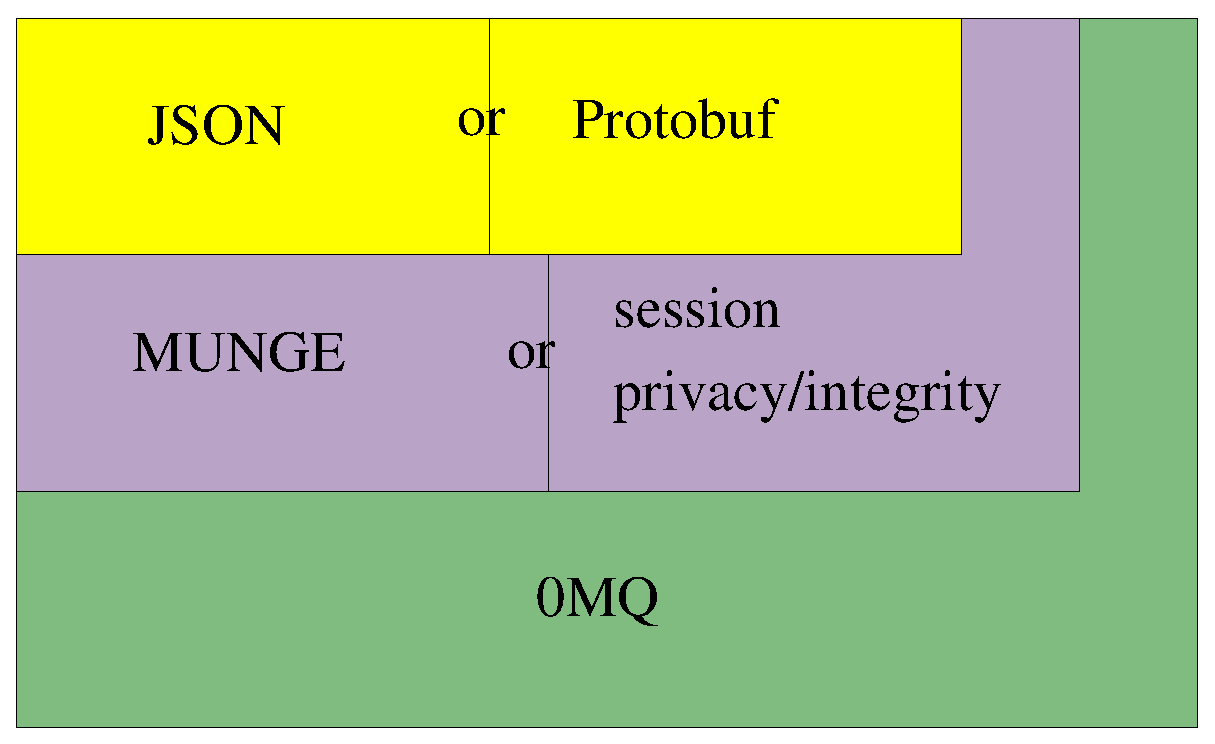
\includegraphics[scale=0.20]{commstk}
\end{center}
\begin{itemize}
  \item{Message handling (2 options)}
  \item{Security (2 options)}
  \item{Message encoding (2 options)}
\end{itemize}
}\end{slide}
% ==========================================================================
\begin{slide}{Message Handling}{\small
  \hfill
  \begin{minipage}{0.5\textwidth}
  {\bf \zMQ}
  \begin{itemize}
    \item{req-rep, pub-sub, push-pull}
    \item{PGM (reliable multicast)}
    \item{multipart message handling}
    \item{support for broker construction}
    \item{user space library}
  \end{itemize}
  \begin{center}
    \begin{minipage}[b]{0.15\linewidth}
    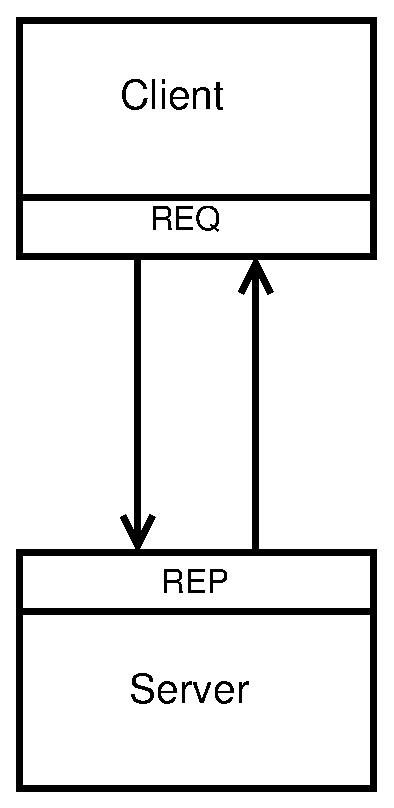
\includegraphics[scale=0.08]{comms_zmq_reqrep}
    \end{minipage}
    \hspace{0.2cm}
    \begin{minipage}[b]{0.3\linewidth}
    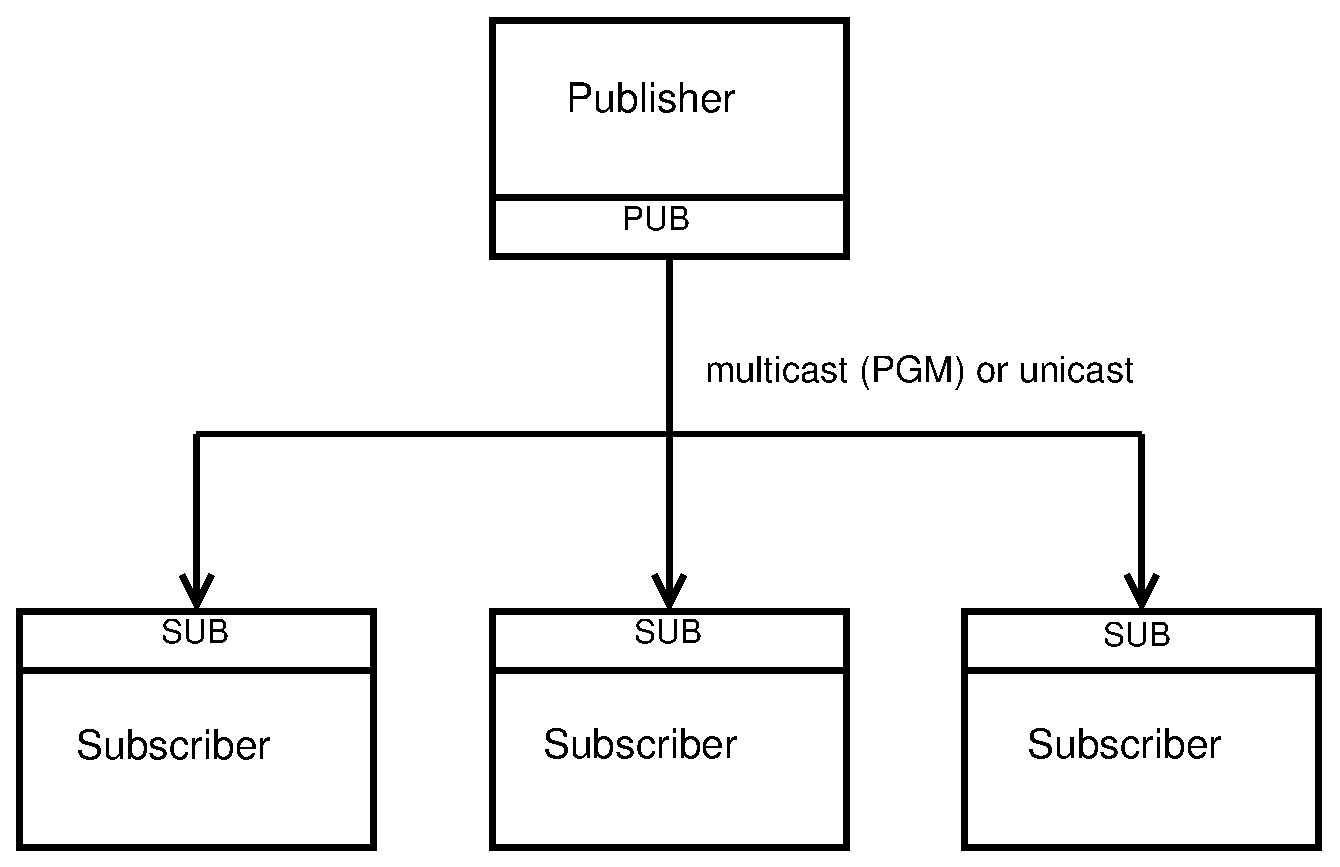
\includegraphics[scale=0.08]{comms_zmq_pubsub}
    \end{minipage}
    \hspace{0.2cm}
    \begin{minipage}[b]{0.3\linewidth}
    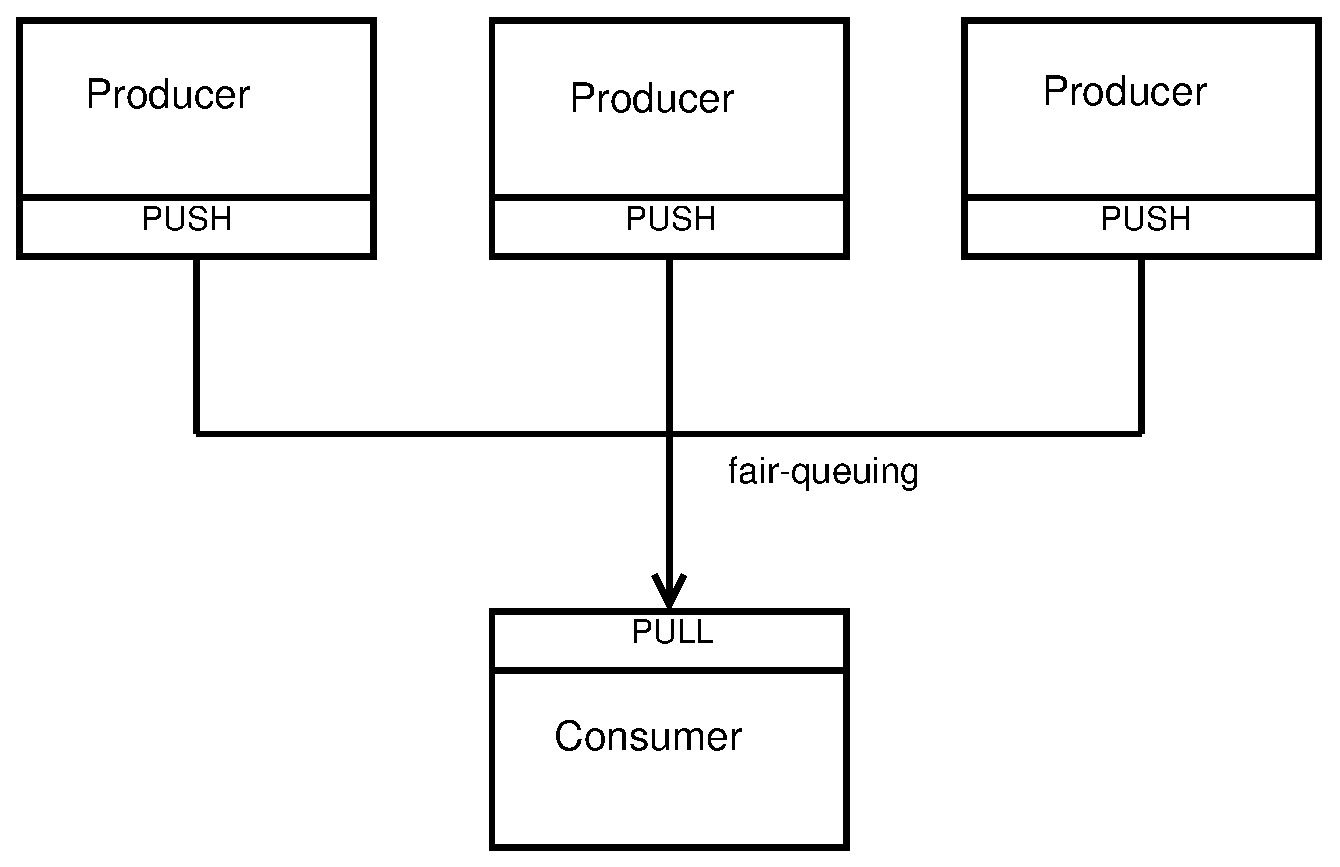
\includegraphics[scale=0.08]{comms_zmq_pushpull}
    \end{minipage}
  \end{center}
  \end{minipage}
  \hfill
  \begin{minipage}{0.45\textwidth}
  {\bf SCTP}
  \begin{itemize}
    \item{message oriented}
    \item{transparent multi-homing}
    \item{multi-streaming}
    \item{N-to-1 associations}
    \item{HMAC check option}
    \item{IETF, in Linux kernel}
  \end{itemize}
  \begin{center}
  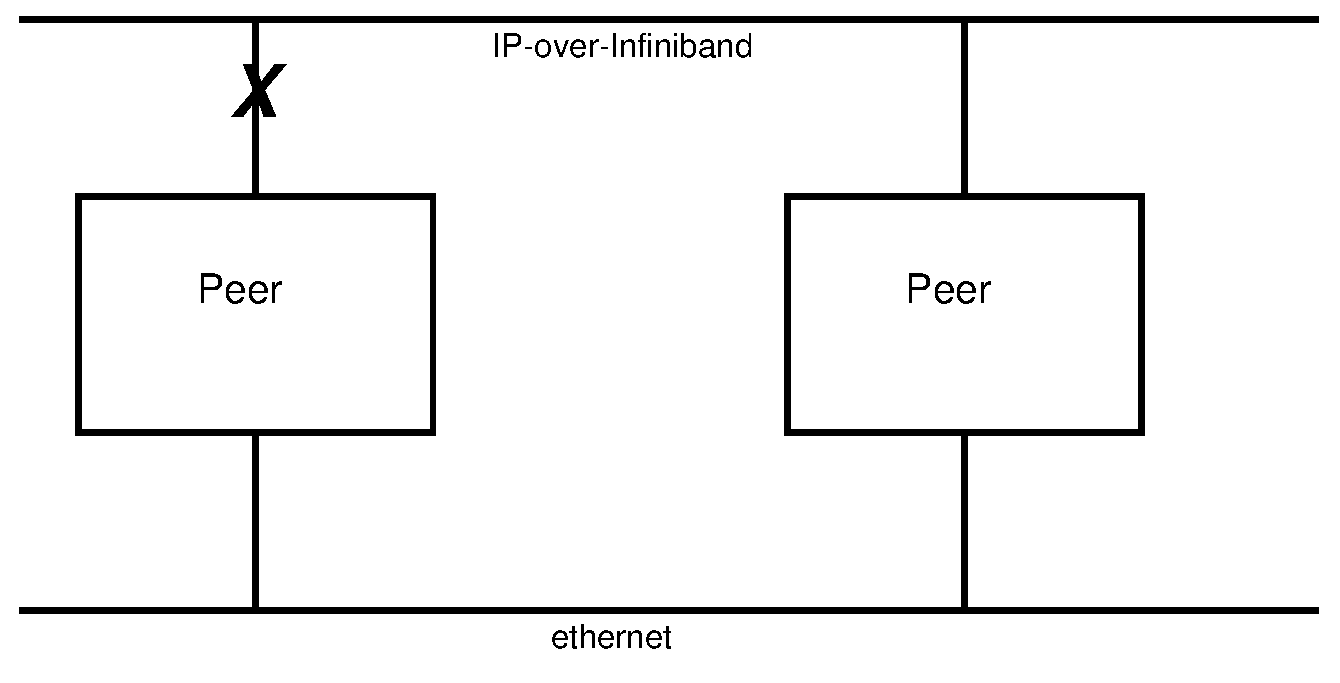
\includegraphics[scale=0.10]{comms_sctp}
  \end{center}
  \end{minipage}
  \hfill
}\end{slide}
% ==========================================================================
\begin{slide}{Security}{\small
  \hfill
  \begin{minipage}{0.5\textwidth}
  {\bf session security context}
  \begin{itemize}
    \item{key assigned by parent}
    \item{integrity, privacy for all}
    \item{parent knows child's key}
    \item{child forgets parent's key}
    \item{useful for pub-sub}
    \item{assumes trust within session}
  \end{itemize}
  \end{minipage}
  \hfill
  \begin{minipage}{0.45\textwidth}
  {\bf MUNGE}
  \begin{itemize}
    \item{key assigned out of band (don't ask)}
    \item{privileged munge daemon signs messages}
    \item{authenticates sender}
    \item{integrity, privacy of payload possible}
  \end{itemize}
  \end{minipage}
  \hfill
}\end{slide}
% ==========================================================================
\begin{slide}{Message Encoding}{\small
  \hfill
  \begin{minipage}{0.5\textwidth}
  {\bf JSON}
  \begin{itemize}
    \item{generated on the fly}
    \item{many language bindings}
    \item{human readable}
    \item{easily extended}
    \item{space-inefficient}
    \item{slow}
  \end{itemize}
  \end{minipage}
  \hfill
  \begin{minipage}{0.45\textwidth}
  {\bf Protocol Buffers}
  \begin{itemize}
    \item{compiled from IDL}
    \item{fewer supported languages}
    \item{machine readable}
    \item{must design for revision}
    \item{space-efficient}
    \item{fast}
  \end{itemize}
  \end{minipage}
  \hfill
}\end{slide}
% ==========================================================================
\begin{slide}{Comms Message Broker (CMB)}{\small
\begin{itemize}
  \item{a distributed service within a comms session}
  \item{launches new sessions}
  \item{manages session membership}
  \item{detect session node failures, and adapt}
  \item{basic event messaging system}
  \item{bootstrap other components}
\end{itemize}
\begin{minipage}[b]{0.18\linewidth}
\fbox{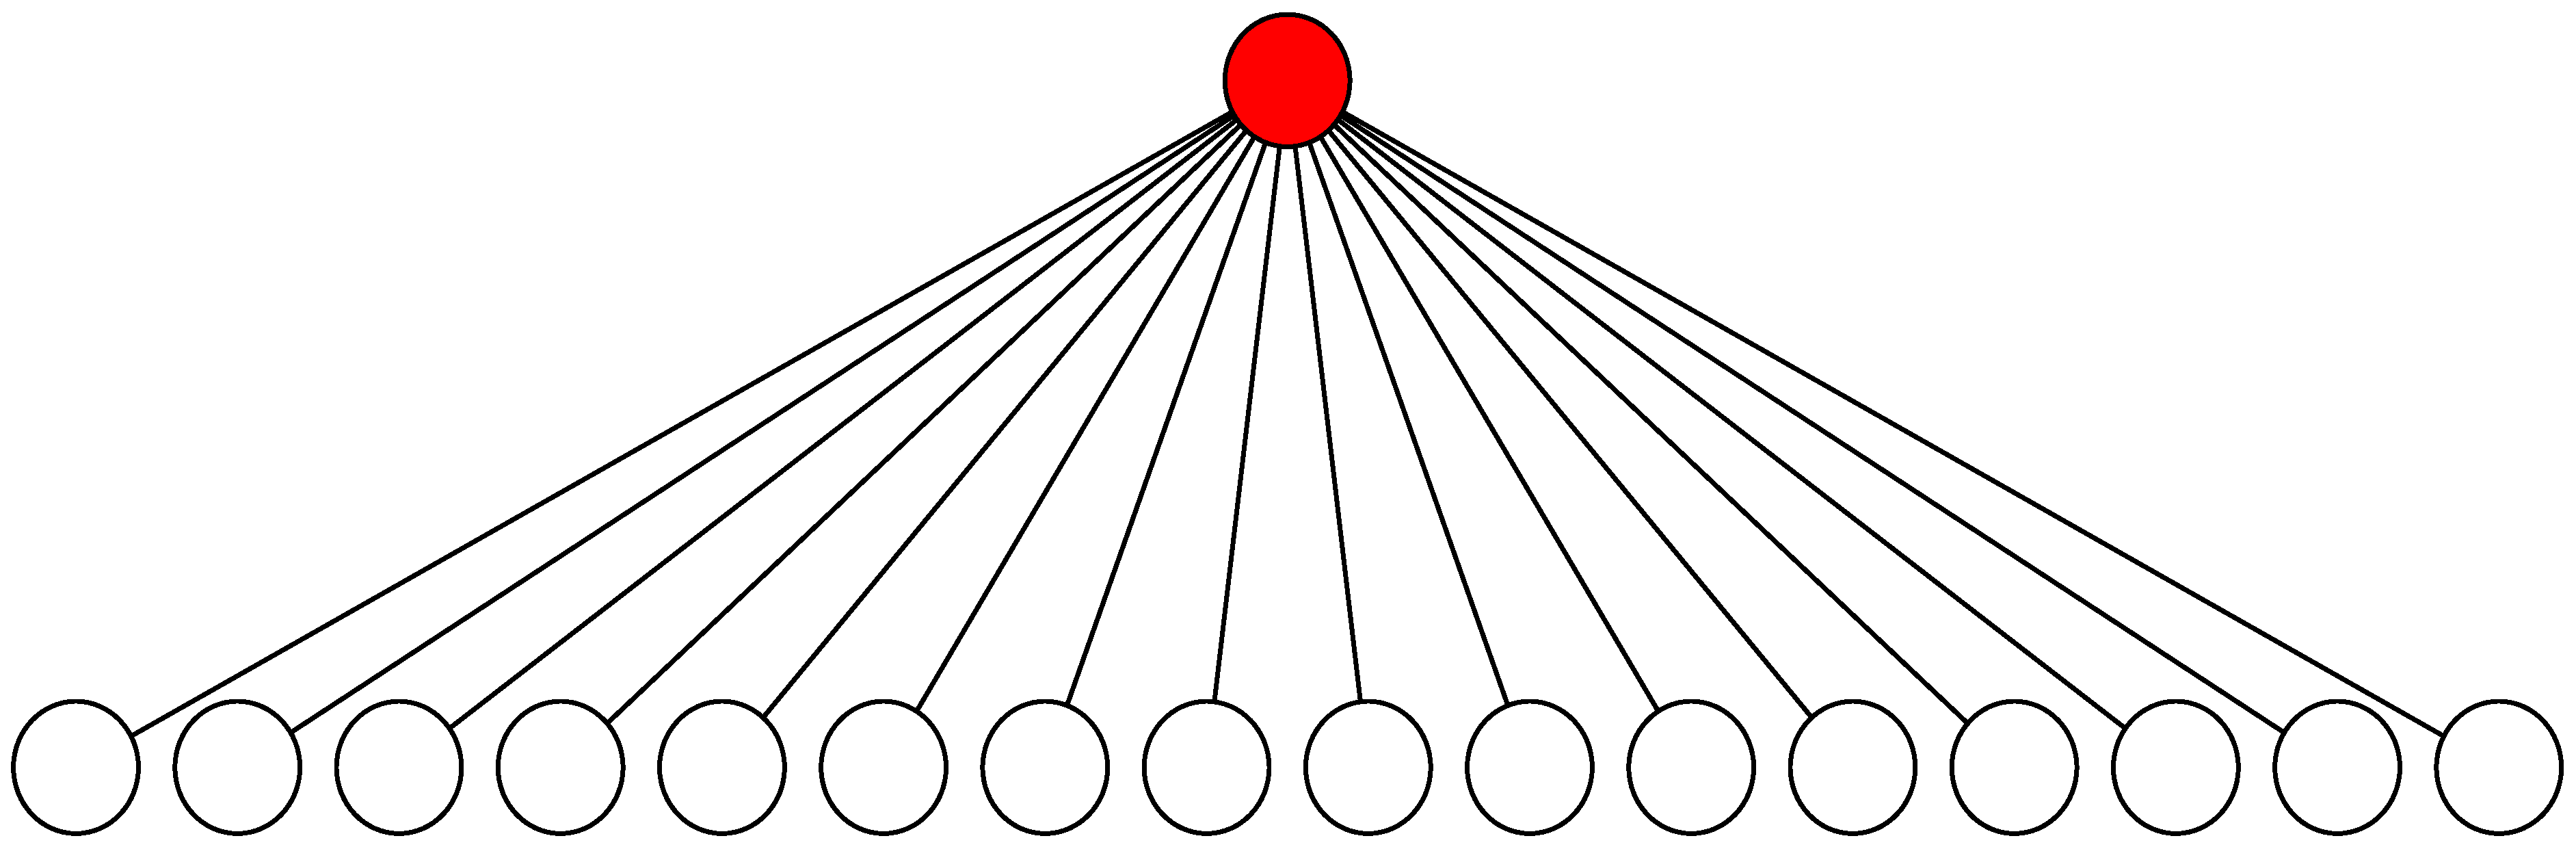
\includegraphics[scale=0.04]{comms_ex1a}}
\end{minipage}
\hspace{0.5cm}
\begin{minipage}[b]{0.18\linewidth}
\fbox{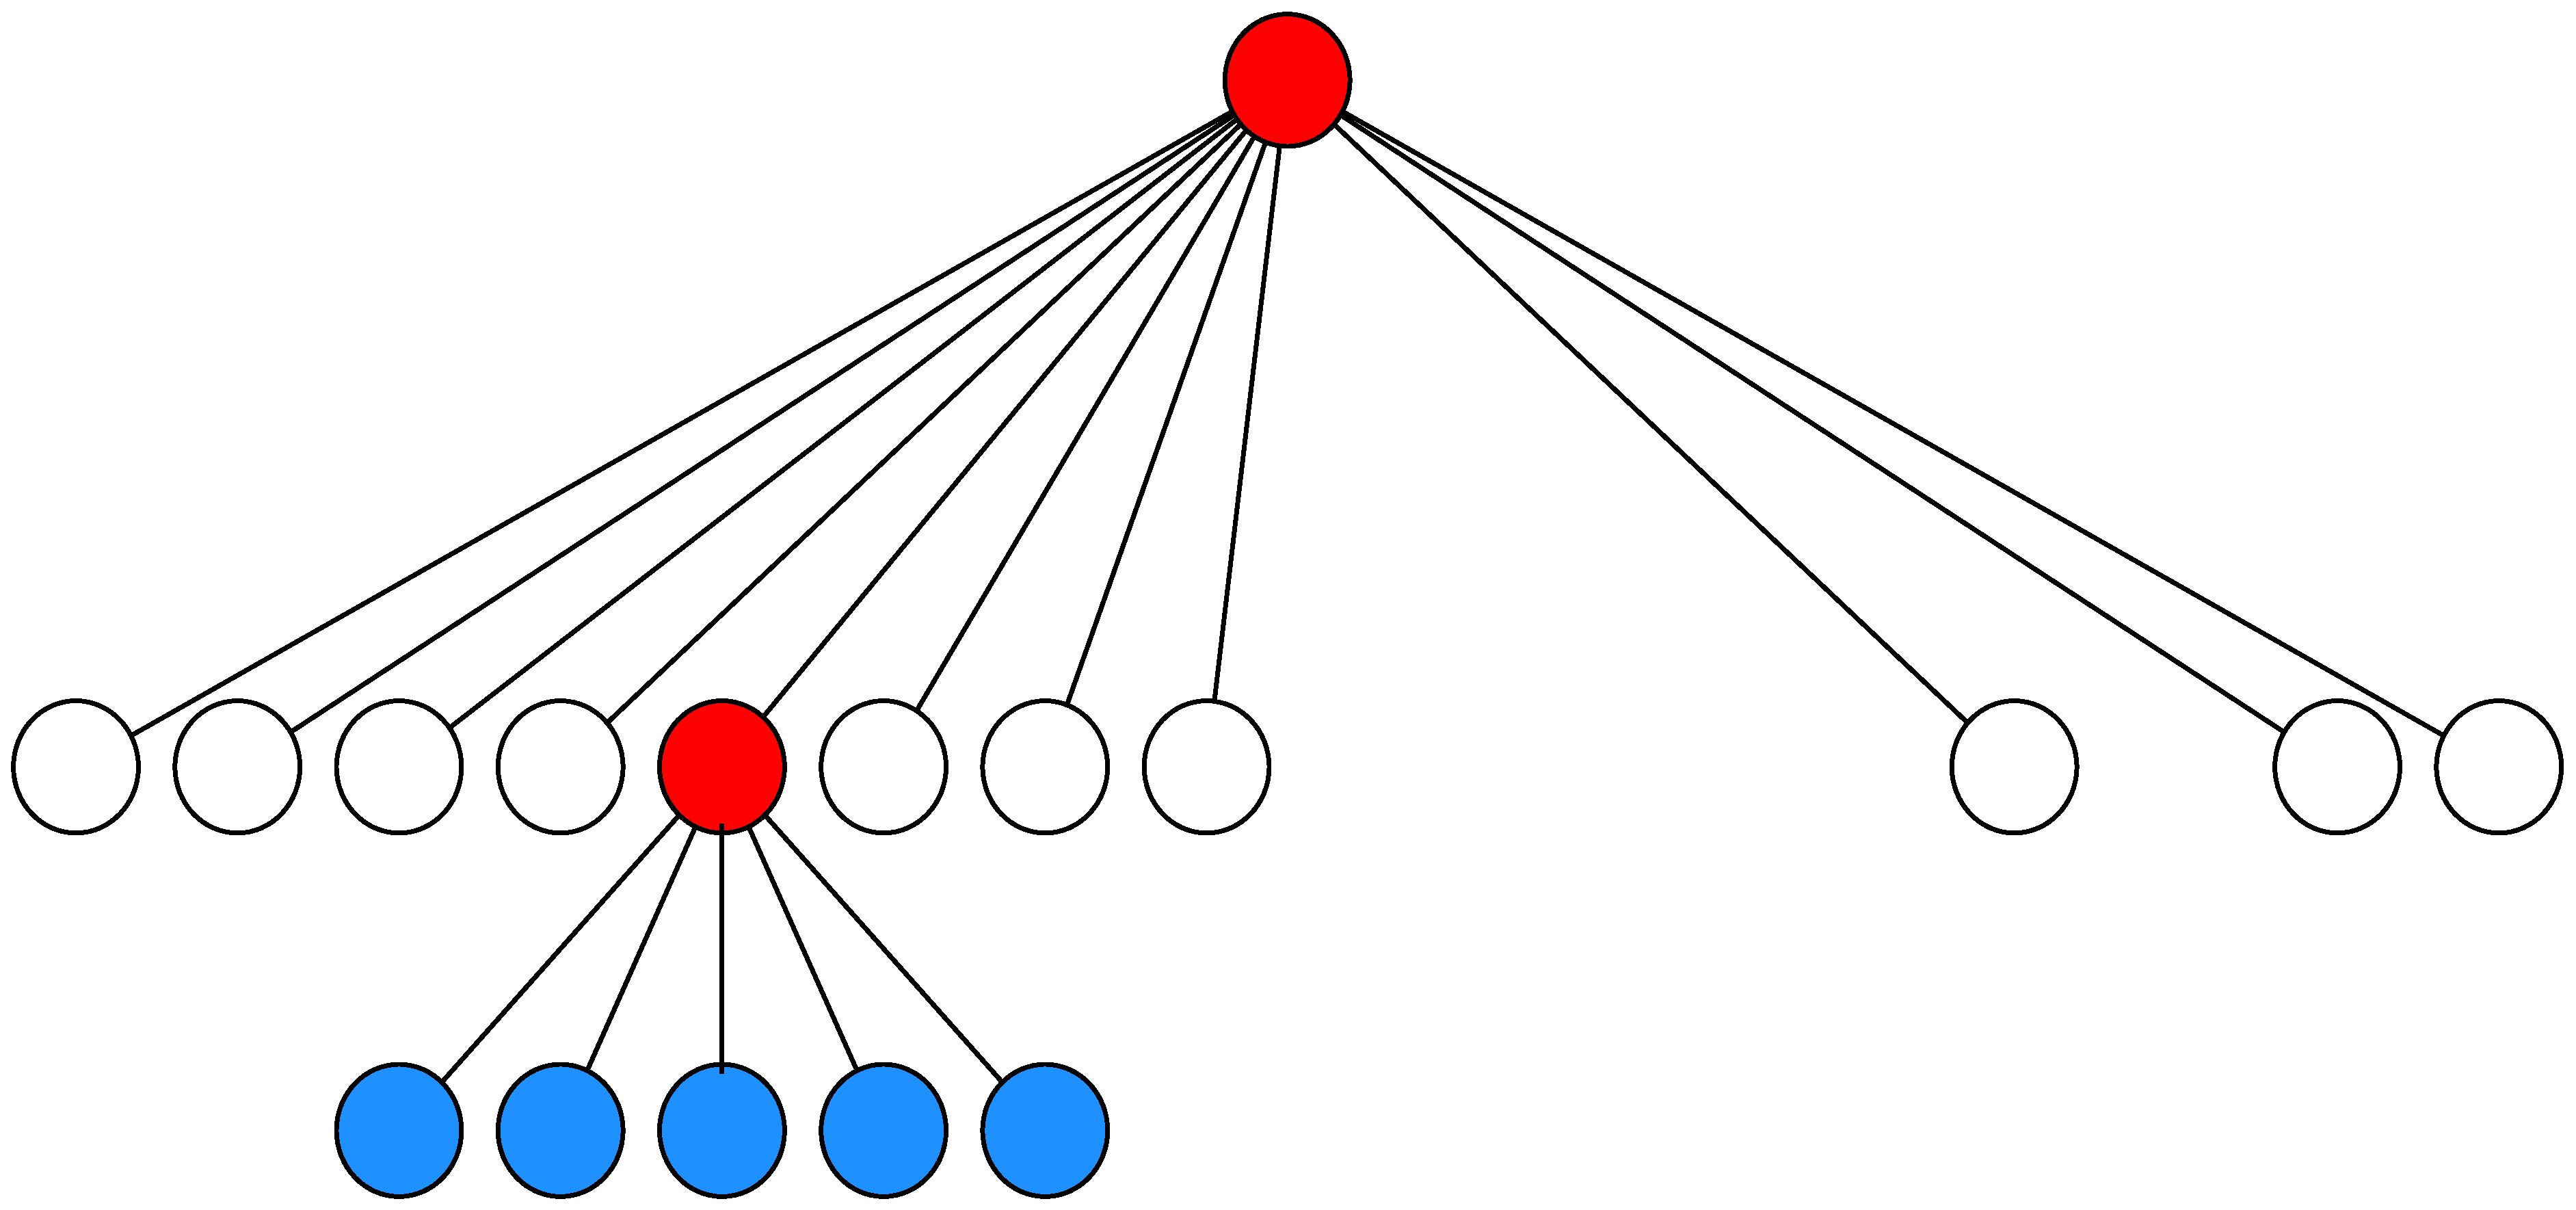
\includegraphics[scale=0.04]{comms_ex1b}}
\end{minipage}
\hspace{0.5cm}
\begin{minipage}[b]{0.18\linewidth}
\fbox{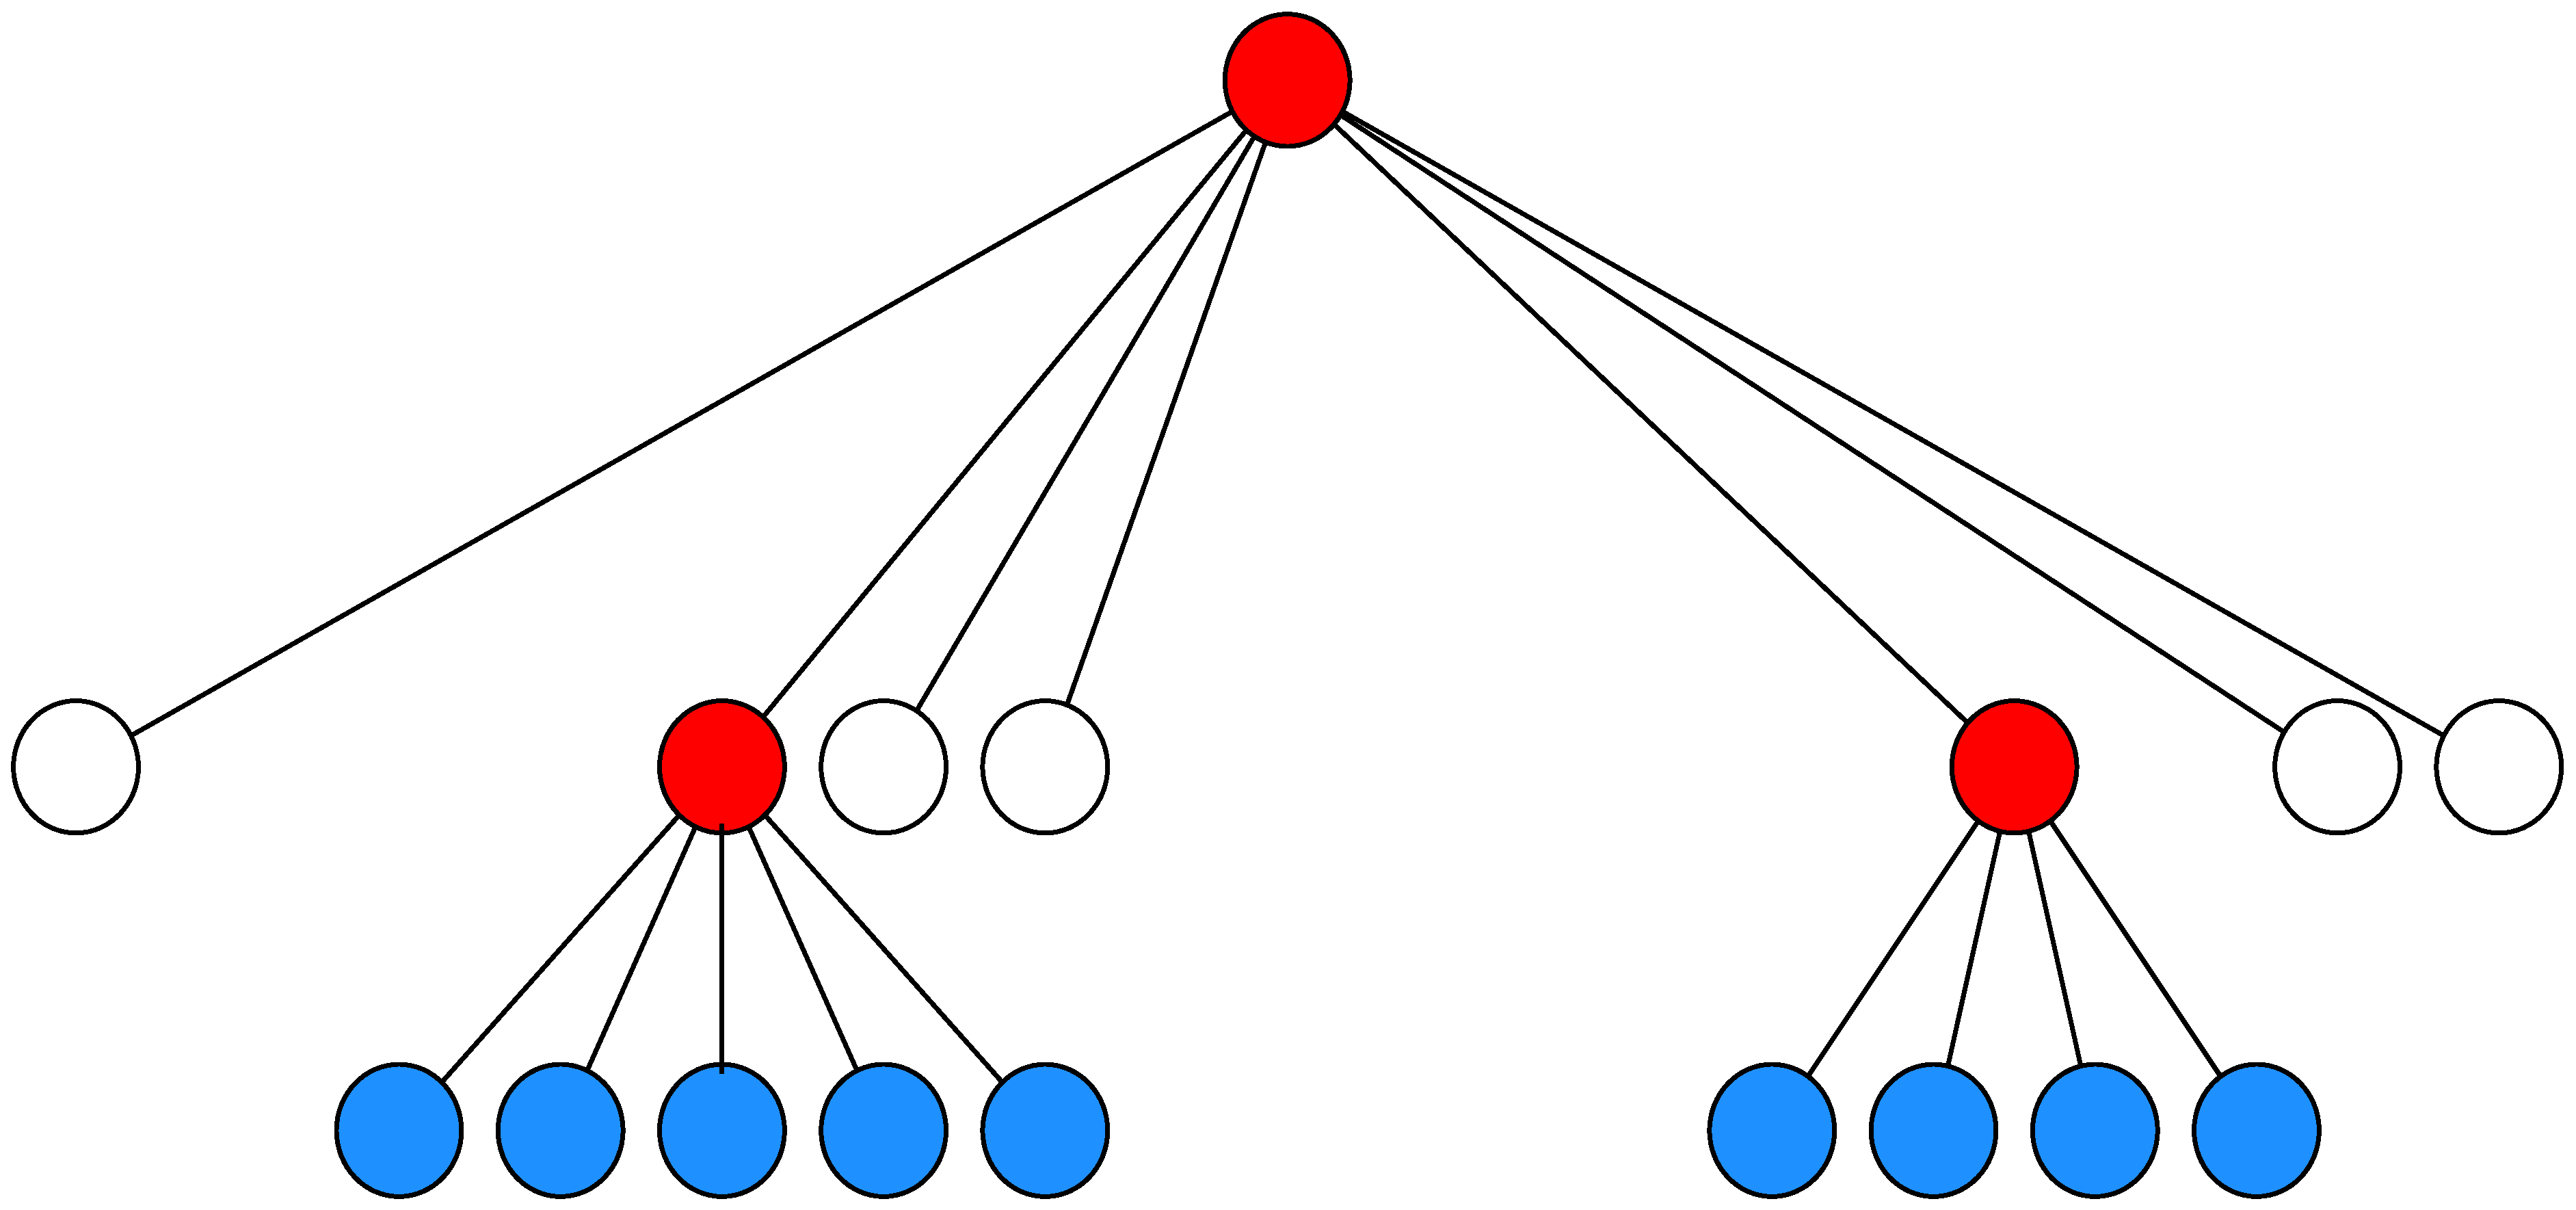
\includegraphics[scale=0.04]{comms_ex1c}}
\end{minipage}
\hspace{0.5cm}
\begin{minipage}[b]{0.18\linewidth}
\fbox{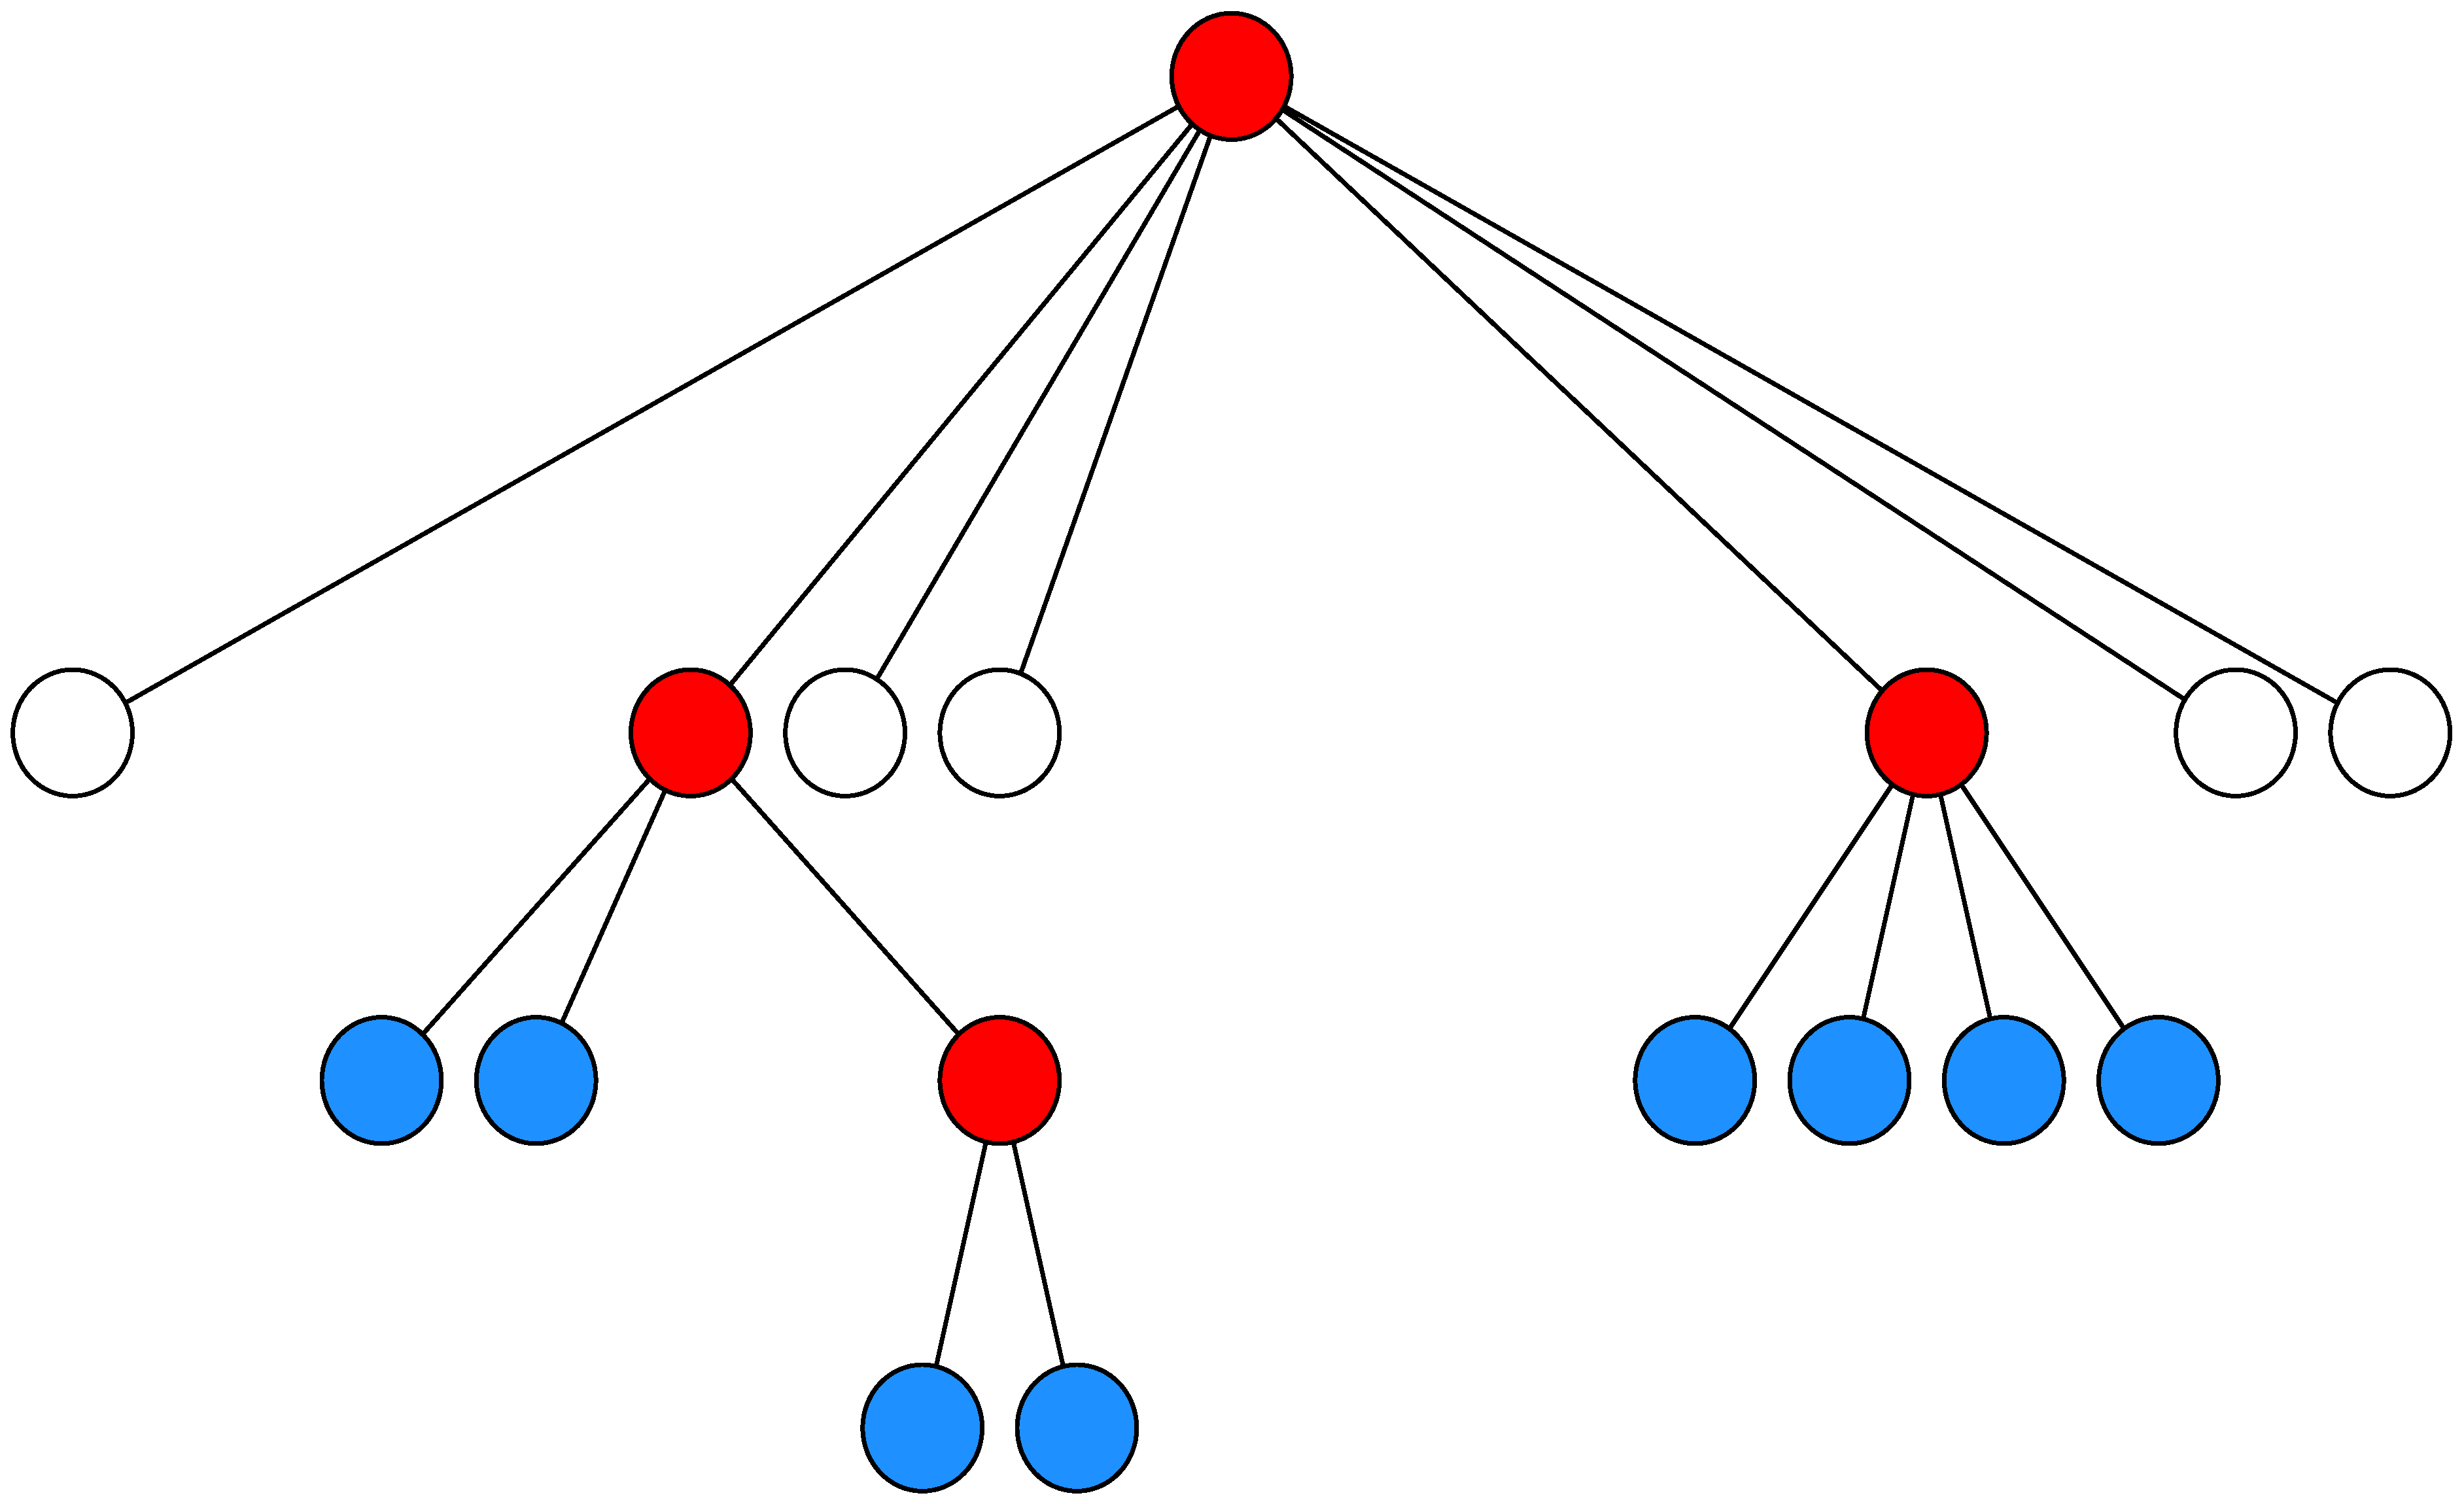
\includegraphics[scale=0.04]{comms_ex1d}}
\end{minipage}
}\end{slide}
% ==========================================================================
\begin{slide}{CMB - more detail}{\small
\begin{itemize}
  \item{distinguished control node (root of tree, gateway)}
  \item{session state K-V store w/ loosely consistent slave caches
	(session key, nodeset, topo, liveness, etc.)}
  \item{pub-sub event messaging $(tag, message)$;\\
	periodic {\tt event.sched.trigger} heartbeat event;\\
	events on state update for slave cache sync}
  \item{liveness monitoring based on forced periodic communication;
	parent can subscribe}
  \item{parent handles session creation/resize/destruction}
  \item{DNS subdomain management}
\end{itemize}
}\end{slide}
% ==========================================================================
\begin{slide}{Reduction Network}{\small
\begin{minipage}{0.50\textwidth}
\begin{itemize}
  \item{tracks CMB topology (including elasticity, fault tolerance)}
  %\item{back-ends on all nodes, internal TBD, front-end" on control node}
  \item{downstream: PGM; upstream: unicast; messages: $(tag, message)$}
  \item{contribs to CMB liveness}
\end{itemize}
\vspace{0.10mm}
\end{minipage}
\begin{minipage}{0.40\textwidth}
\begin{center}
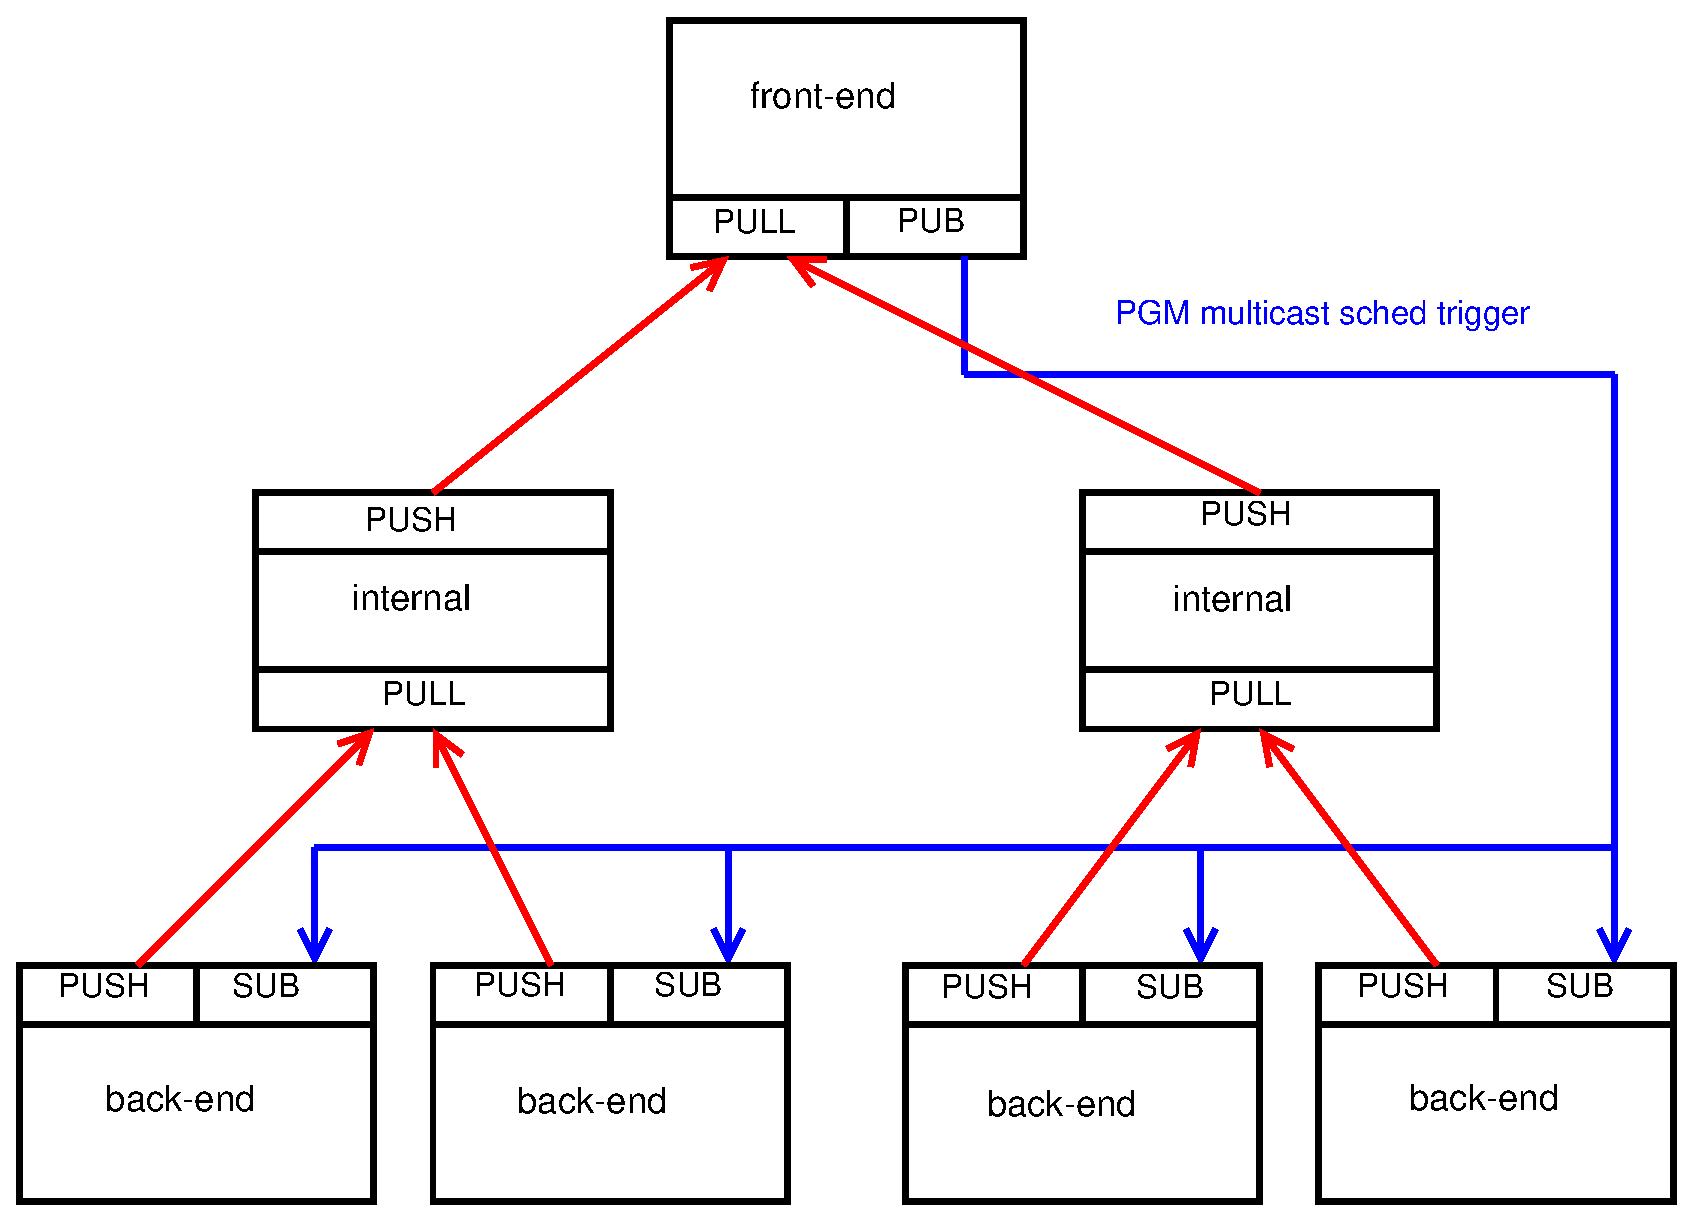
\includegraphics[scale=0.20]{comms_zmq_reduct}
\end{center}
\end{minipage}
\begin{itemize}
  \item{shared by multiple \ngrm\ components}
  \item{plugins with service activation, UNIX domain sockets}
  \item{co-design with runtime thrust, could be other TB\={O}Ns}
\end{itemize}
}\end{slide}
% ==========================================================================
\begin{slide}{Fault Tolerance}{\small
\begin{itemize}
  \item{{\em FT is a significant design activity!}}
  \item{high stakes: losing the root job is bad}
  \item{rebooting nodes know how to rejoin root session}
  \item{CMB events notify when session state changes\\
	(nodeset, liveness, topo)}
  \item{CMB state is replicated in slave caches}
  \item{parent monitors control node and orchestrates recovery}
\end{itemize}
}\end{slide}
% ==========================================================================
\begin{slide}{Session Overview}{\small
\begin{itemize}
  \item[\S1-4]{{\gray {\em overview} (Jim)}}
  \item[\S5]{{\gray {\em comms framework} (Jim)}}
  \item[\S6.1-6]{{\em resource management} (Mark)}
  \item[\S6.7]{{\em scheduler} (Don)}
  \item[\S7]{{\em monitoring} (Jim)}
  \item[\S8]{{\em runtime} (Dong)}
\end{itemize}
}\end{slide}
% ==========================================================================
%\part{resource management}
% ==========================================================================
%\part{scheduler}
% ==========================================================================
\part{monitoring}
% ==========================================================================
\begin{slide}{Monitoring}{\small
\begin{minipage}{0.40\textwidth}
Overview:
\begin{itemize}
  \item{job-customizable monitoring domain}
  \item{health $\Longrightarrow$ res DB}
  \item{faults $\Longrightarrow$ job DB}
  \item{raw data $\Longrightarrow$ log DB}
\end{itemize}
\end{minipage}
\hfill
\begin{minipage}{0.50\textwidth}
Components:
\begin{itemize}
  \item{plugin framework}
  \item{log database (external)}
  \item{fault notification system}
  \item{enterprise mon (external)}
\end{itemize}
\end{minipage}
\vspace{0.5cm}
\begin{center}
\fbox{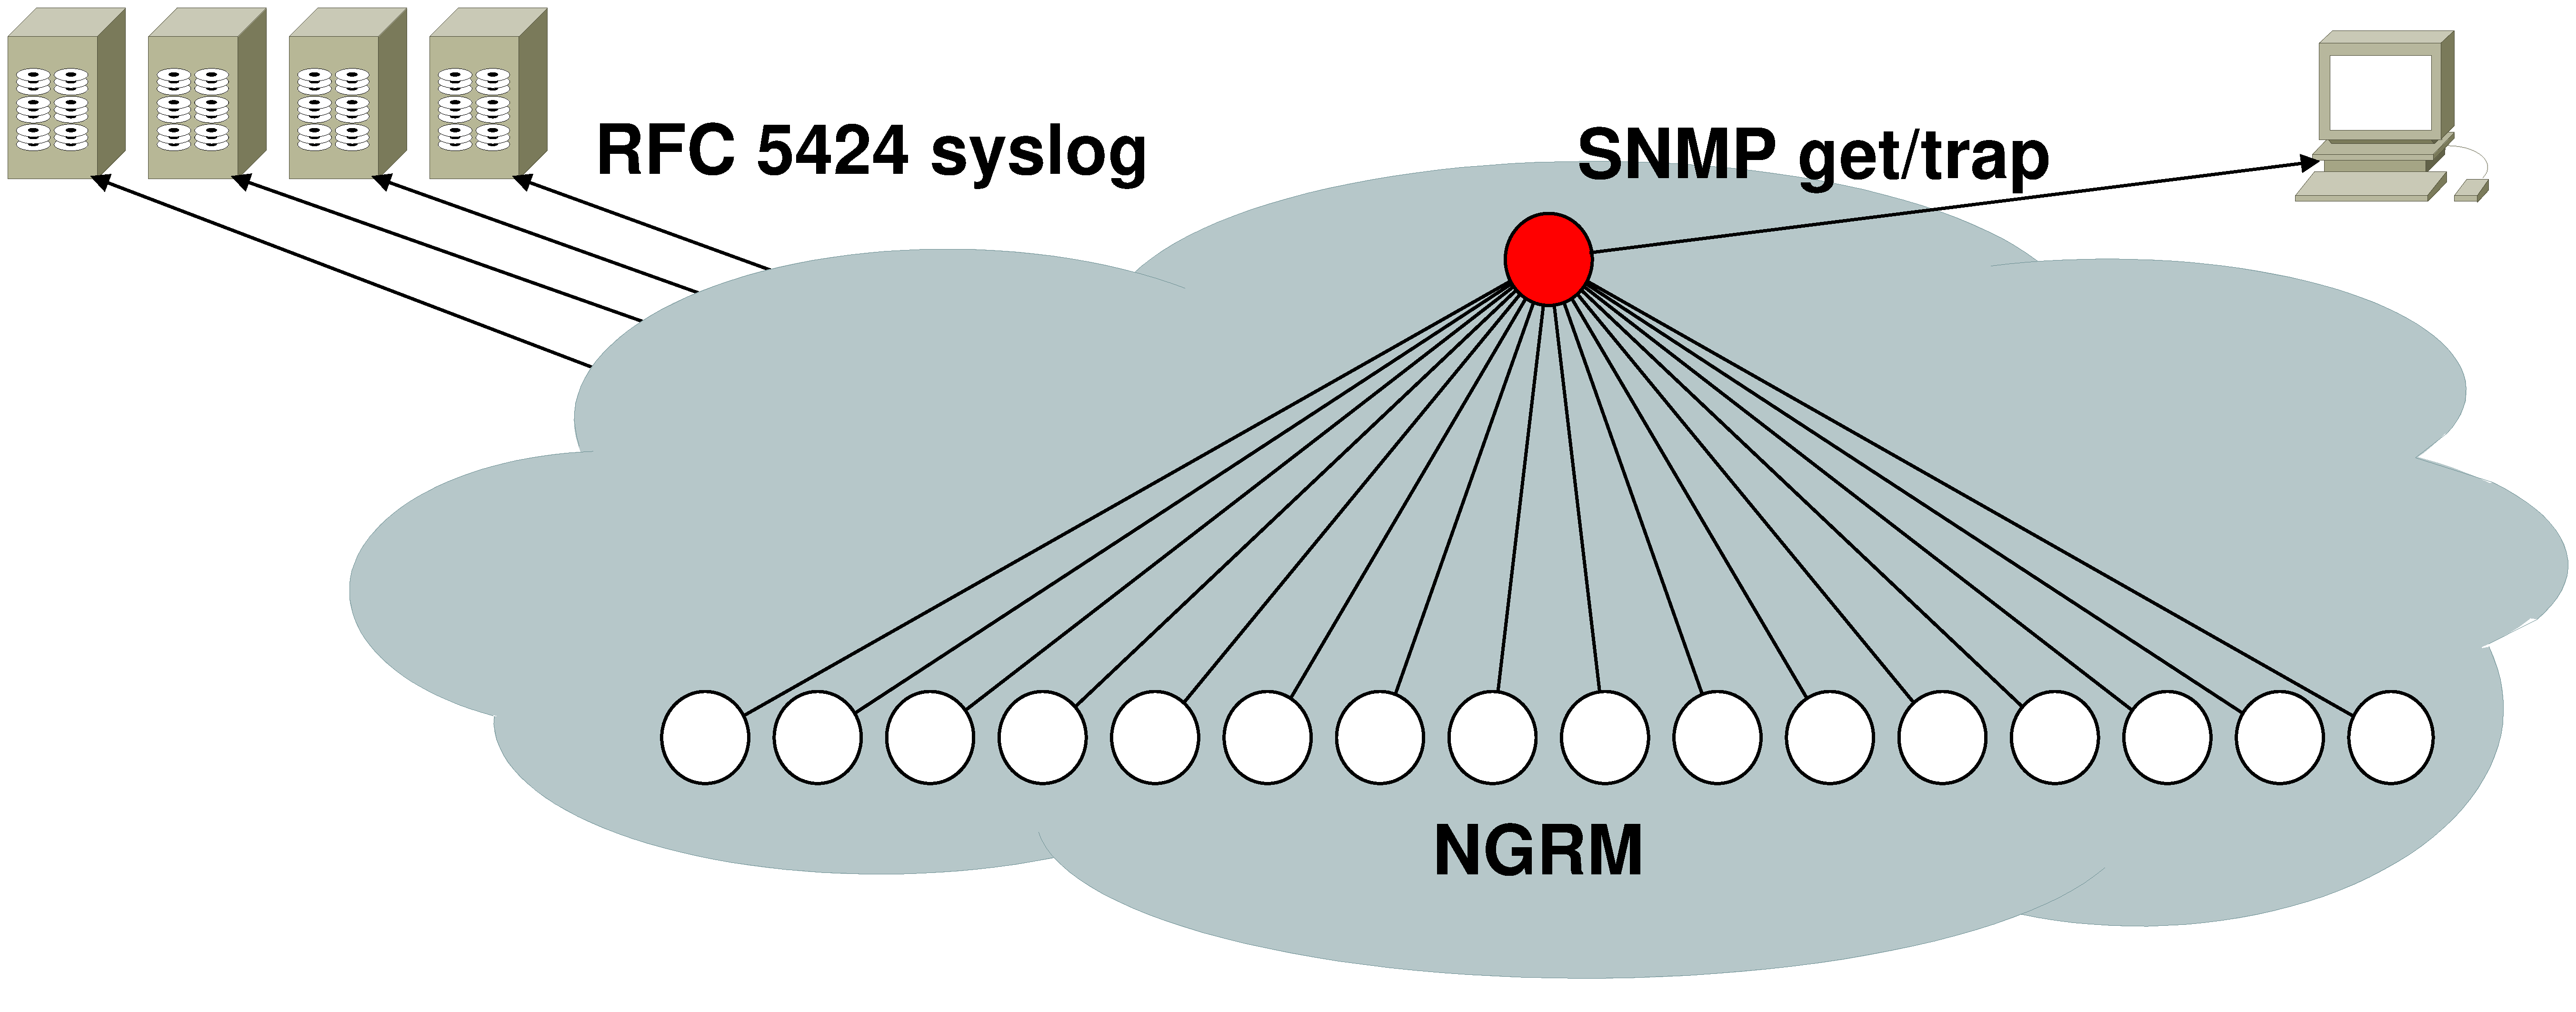
\includegraphics[scale=0.07]{mon_iface}}
\end{center}
}\end{slide}
% ==========================================================================
\begin{slide}{Plugin Framework}{\small
\begin{center}
\begin{minipage}[b]{0.4\linewidth}
\fbox{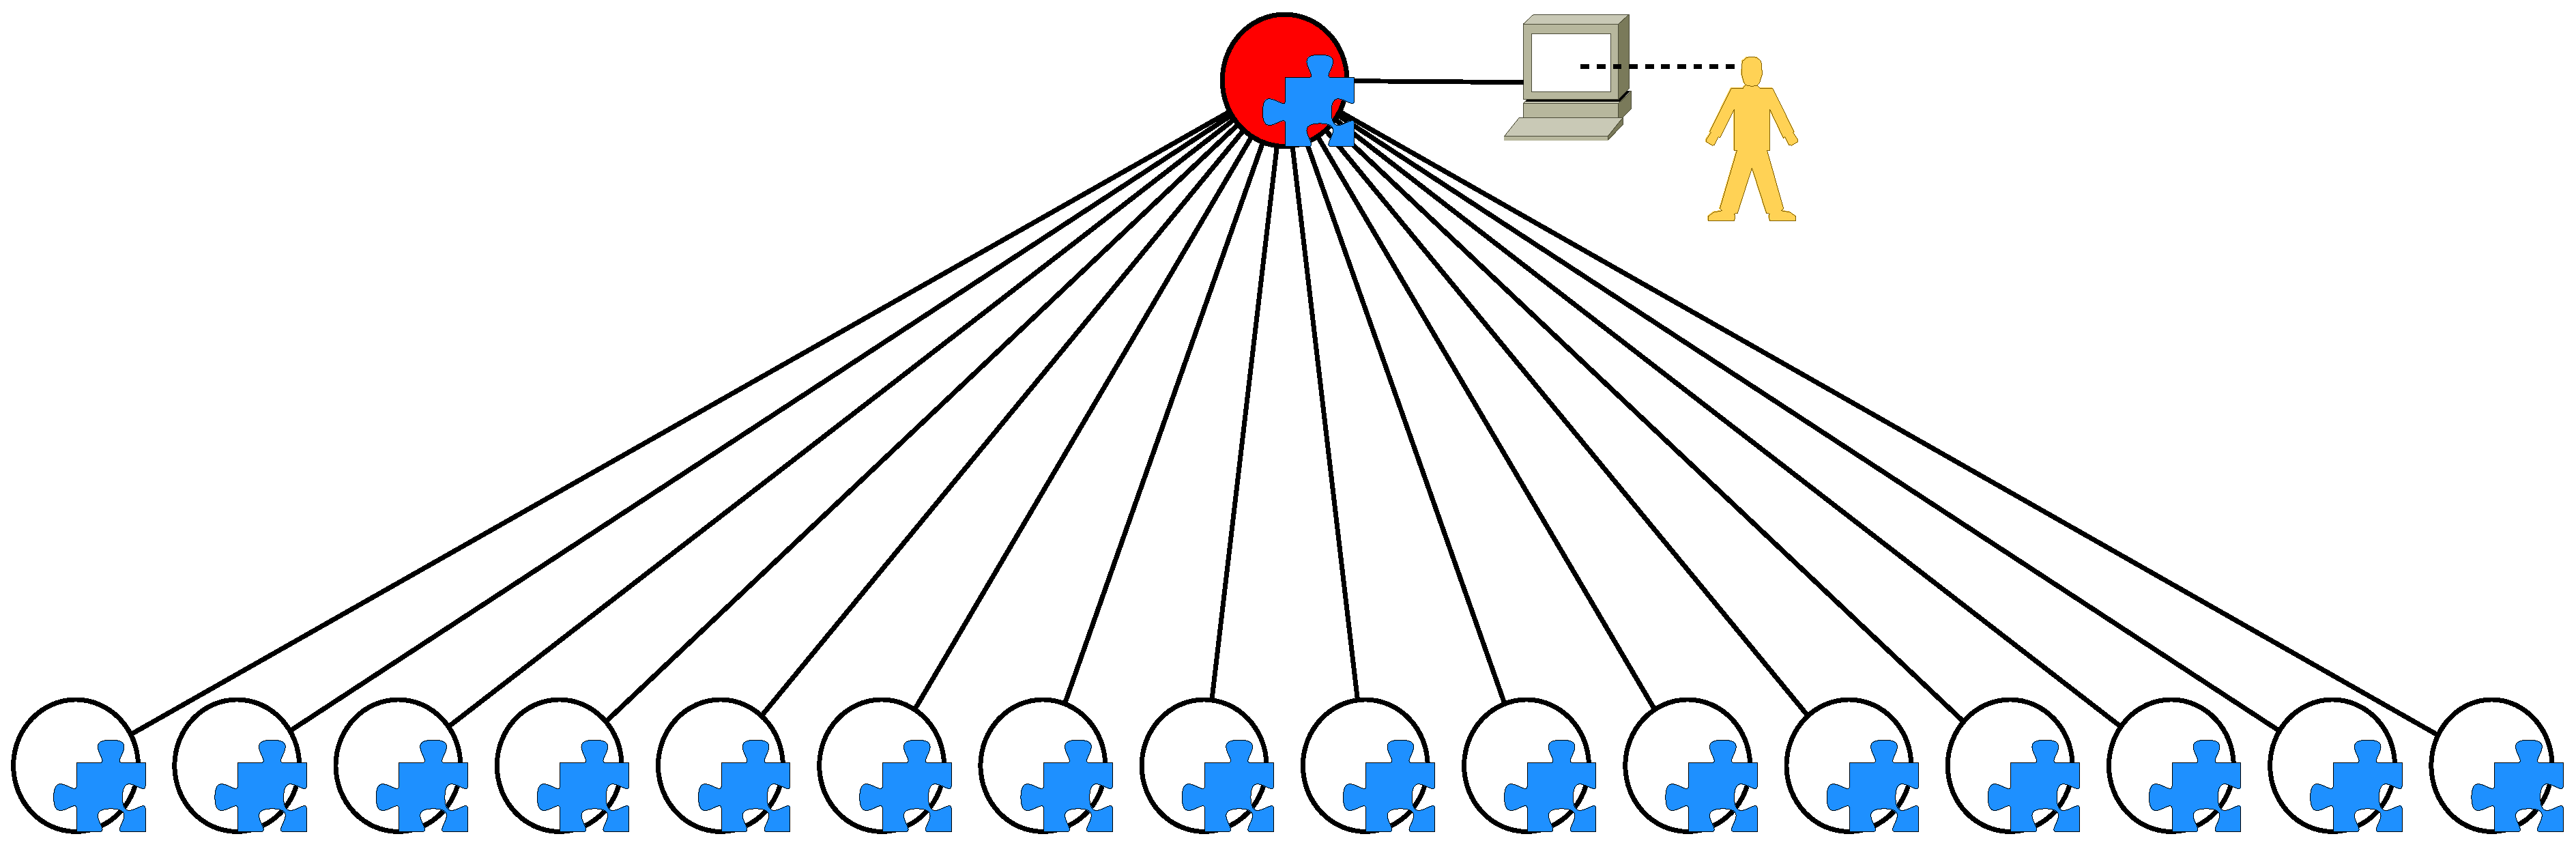
\includegraphics[scale=0.07]{mon_ex1a}}
\end{minipage}
\hspace{0.5cm}
\begin{minipage}[b]{0.4\linewidth}
\fbox{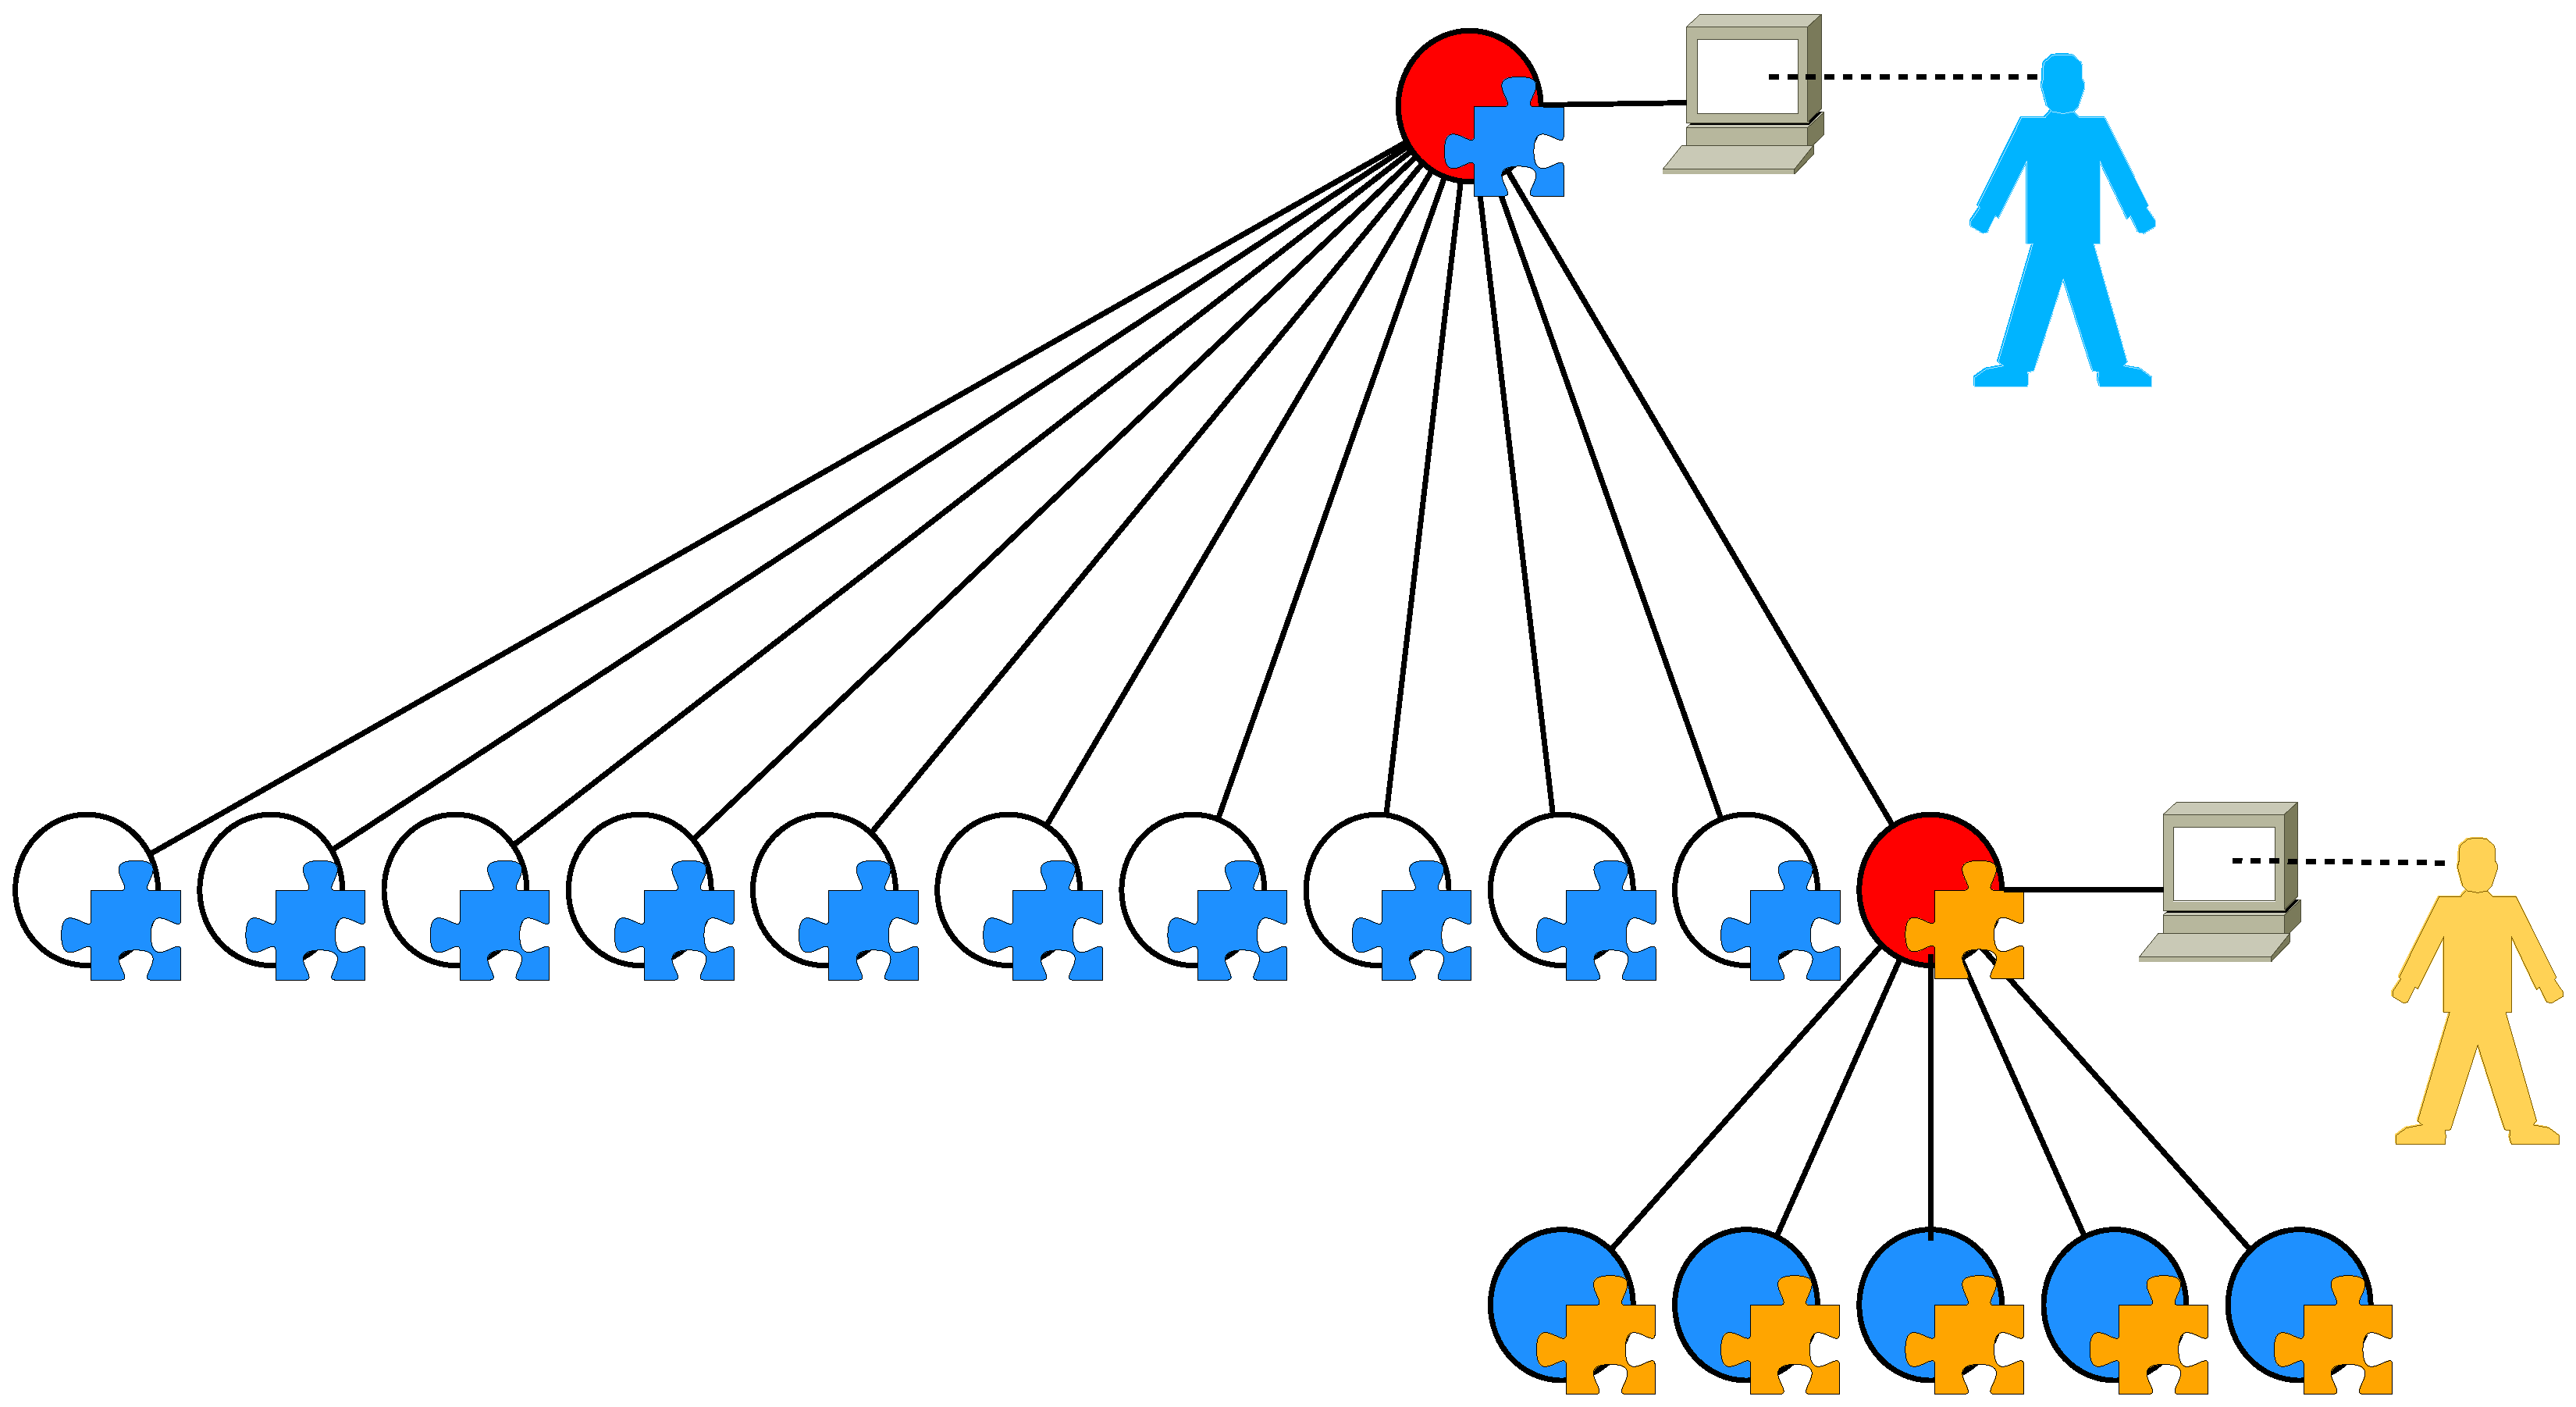
\includegraphics[scale=0.07]{mon_ex1b}}
\end{minipage}
\end{center}
\begin{itemize}
  \item{plugin stack uses comms reduction network}
  \item{source(): get raw data, sync sched event ($T=$ tunable)}
  \item{reduction(): combine raw data}
  \item{sink(): update res DB}
  \item{functions can generate faults, log entries}
\end{itemize}
}\end{slide}
% ==========================================================================
\begin{slide}{Log database (external)}{\small
\begin{itemize}
  \item{comprehensive, schemaless, site-wide store}
  \item{high insertion rate}
  \item{large storage capacity}
  \item{scalable queries}
  \item{facilitates post-mortem analysis, beyond job record}
  \item{RFC 5424 syslog STRUCTURED-DATA enhancement}
\end{itemize}
}\end{slide}
% ==========================================================================
\begin{slide}{Fault notification system}{\small
\begin{itemize}
  \item{Foof!}
\end{itemize}
}\end{slide}
% ==========================================================================
\begin{slide}{Enterprise monitoring system (external)}{\small
\begin{itemize}
  \item{Foof!}
\end{itemize}
}\end{slide}
% ==========================================================================
\begin{slide}{Session Overview}{\small
\begin{itemize}
  \item[\S1-4]{{\gray {\em overview} (Jim)}}
  \item[\S5]{{\gray {\em comms framework} (Jim)}}
  \item[\S6.1-6]{{\gray {\em resource management} (Mark)}}
  \item[\S6.7]{{\gray {\em scheduler} (Don)}}
  \item[\S7]{{\gray {\em monitoring} (Jim)}}
  \item[\S8]{{\em runtime} (Dong)}
\end{itemize}
}\end{slide}
% ==========================================================================
%\part{runtime}
% ==========================================================================
\end{document}
